% This is "sig-alternate.tex" V2.1 April 2013
% This file should be compiled with V2.5 of "sig-alternate.cls" May 2012
%
% This example file demonstrates the use of the 'sig-alternate.cls'
% V2.5 LaTeX2e document class file. It is for those submitting
% articles to ACM Conference Proceedings WHO DO NOT WISH TO
% STRICTLY ADHERE TO THE SIGS (PUBS-BOARD-ENDORSED) STYLE.
% The 'sig-alternate.cls' file will produce a similar-looking,
% albeit, 'tighter' paper resulting in, invariably, fewer pages.
%
% ----------------------------------------------------------------------------------------------------------------
% This .tex file (and associated .cls V2.5) produces:
%       1) The Permission Statement
%       2) The Conference (location) Info information
%       3) The Copyright Line with ACM data
%       4) NO page numbers
%
% as against the acm_proc_article-sp.cls file which
% DOES NOT produce 1) thru' 3) above.
%
% Using 'sig-alternate.cls' you have control, however, from within
% the source .tex file, over both the CopyrightYear
% (defaulted to 200X) and the ACM Copyright Data
% (defaulted to X-XXXXX-XX-X/XX/XX).
% e.g.
% \CopyrightYear{2007} will cause 2007 to appear in the copyright line.
% \crdata{0-12345-67-8/90/12} will cause 0-12345-67-8/90/12 to appear in the copyright line.
%
% ---------------------------------------------------------------------------------------------------------------
% This .tex source is an example which *does* use
% the .bib file (from which the .bbl file % is produced).
% REMEMBER HOWEVER: After having produced the .bbl file,
% and prior to final submission, you *NEED* to 'insert'
% your .bbl file into your source .tex file so as to provide
% ONE 'self-contained' source file.
%
% ================= IF YOU HAVE QUESTIONS =======================
% Questions regarding the SIGS styles, SIGS policies and
% procedures, Conferences etc. should be sent to
% Adrienne Griscti (griscti@acm.org)
%
% Technical questions _only_ to
% Gerald Murray (murray@hq.acm.org)
%
% Technical questions related to COCO/BBOB to bbob@lri.fr
% ===============================================================
%
% For tracking purposes - this is V2.0 - May 2012

\documentclass{sig-alternate}

\usepackage{graphicx}
\usepackage{rotating}
\usepackage[dvipsnames]{xcolor}  % color is sufficient
%\usepackage[hidelinks]{hyperref} % make COCO papers clickable


\pdfpagewidth=8.5in
\pdfpageheight=11in
\special{papersize=8.5in,11in}

    \renewcommand{\topfraction}{1}	% max fraction of floats at top
    \renewcommand{\bottomfraction}{1} % max fraction of floats at bottom
    %   Parameters for TEXT pages (not float pages):
    \setcounter{topnumber}{3}
    \setcounter{bottomnumber}{3}
    \setcounter{totalnumber}{3}     % 2 may work better
    \setcounter{dbltopnumber}{4}    % for 2-column pages
    \renewcommand{\dbltopfraction}{1}	% fit big float above 2-col. text
    \renewcommand{\textfraction}{0.0}	% allow minimal text w. figs
    %   Parameters for FLOAT pages (not text pages):
    \renewcommand{\floatpagefraction}{0.80}	% require fuller float pages
	% N.B.: floatpagefraction MUST be less than topfraction !!
    \renewcommand{\dblfloatpagefraction}{0.7}	% require fuller float pages

%%%%%%%%%%%%%%%%%%%%%%   END OF PREAMBLE   %%%%%%%%%%%%%%%%%%%%%%%%%%%%%%%%%%%%

%%%%%%%%%%%%%%%%%%%%%%%%%%%%%%%%%%%%%%%%%%%%%%%%%%%%%%%%%%%%%%%%%%%%%%%%%%%%%%%
%%%%%%%%% TO BE EDITED %%%%%%%%%%%%%%%%%%%%%%%%%%%%%%%%%%%%%%%%%%%%%%%%%%%%%%%%
%%%%%%%%%%%%%%%%%%%%%%%%%%%%%%%%%%%%%%%%%%%%%%%%%%%%%%%%%%%%%%%%%%%%%%%%%%%%%%%
% rungeneric.py writes data into a subfolder of ppdata
\newcommand{\bbobdatapath}{ppdata/} % default output folder of rungeneric.py
\input{\bbobdatapath bbob_pproc_commands.tex} % provide default of algname and algfolder
% \renewcommand{\algname}{MYNAME}  % name of algorithm as it should appear in the text
% \renewcommand{\algfolder}{ABC/} % subfolder of \bbobdatapath for processed algorithm
%%%%%%%%%%%%%%%%%%%%%%%%%%%%%%%%%%%%%%%%%%%%%%%%%%%%%%%%%%%%%%%%%%%%%%%%%%%%%%%
%%%%%%%%%%%%%%%%%%%%%%%%%%%%%%%%%%%%%%%%%%%%%%%%%%%%%%%%%%%%%%%%%%%%%%%%%%%%%%%
%%%%%%%%%%%%%%%%%%%%%%%%%%%%%%%%%%%%%%%%%%%%%%%%%%%%%%%%%%%%%%%%%%%%%%%%%%%%%%%
\graphicspath{{\bbobdatapath\algfolder}}

\newcommand{\DIM}{\ensuremath{\mathrm{DIM}}}
\newcommand{\aRT}{\ensuremath{\mathrm{aRT}}}
\newcommand{\FEvals}{\ensuremath{\mathrm{FEvals}}}
\newcommand{\nruns}{\ensuremath{\mathrm{Nruns}}}
\newcommand{\Dfb}{\ensuremath{\Delta f_{\mathrm{best}}}}
\newcommand{\Df}{\ensuremath{\Delta f}}
\newcommand{\nbFEs}{\ensuremath{\mathrm{\#FEs}}}
\newcommand{\fopt}{\ensuremath{f_\mathrm{opt}}}
\newcommand{\ftarget}{\ensuremath{f_\mathrm{t}}}
\newcommand{\CrE}{\ensuremath{\mathrm{CrE}}}
\newcommand{\change}[1]{{\color{red} #1}}

\begin{document}
%
% --- Author Metadata here ---
\conferenceinfo{GECCO'13,} {July 6-10, 2013, Amsterdam, The Netherlands.}
\CopyrightYear{2013}
\crdata{TBA}
\clubpenalty=10000
\widowpenalty = 10000
% --- End of Author Metadata ---

\title{Black-Box Optimization Benchmarking Template for Noiseless Function
Testbed
% \titlenote{If needed}
}
\subtitle{Draft version
\titlenote{Submission deadline: March 28th.}}
%Camera-ready paper due April 17th.}}

%
% You need the command \numberofauthors to handle the 'placement
% and alignment' of the authors beneath the title.
%
% For aesthetic reasons, we recommend 'three authors at a time'
% i.e. three 'name/affiliation blocks' be placed beneath the title.
%
% NOTE: You are NOT restricted in how many 'rows' of
% "name/affiliations" may appear. We just ask that you restrict
% the number of 'columns' to three.
%
% Because of the available 'opening page real-estate'
% we ask you to refrain from putting more than six authors
% (two rows with three columns) beneath the article title.
% More than six makes the first-page appear very cluttered indeed.
%
% Use the \alignauthor commands to handle the names
% and affiliations for an 'aesthetic maximum' of six authors.
% Add names, affiliations, addresses for
% the seventh etc. author(s) as the argument for the
% \additionalauthors command.
% These 'additional authors' will be output/set for you
% without further effort on your part as the last section in
% the body of your article BEFORE References or any Appendices.

\numberofauthors{1} %  in this sample file, there are a *total*
% of EIGHT authors. SIX appear on the 'first-page' (for formatting
% reasons) and the remaining two appear in the \additionalauthors section.
%
\author{
% You can go ahead and credit any number of authors here,
% e.g. one 'row of three' or two rows (consisting of one row of three
% and a second row of one, two or three).
%
% The command \alignauthor (no curly braces needed) should
% precede each author name, affiliation/snail-mail address and
% e-mail address. Additionally, tag each line of
% affiliation/address with \affaddr, and tag the
% e-mail address with \email.
%
% 1st. author
\alignauthor
Forename Name\\ %\titlenote{Dr.~Trovato insisted his name be first.}\\
%       \affaddr{Institute for Clarity in Documentation}\\
%       \affaddr{1932 Wallamaloo Lane}\\
%       \affaddr{Wallamaloo, New Zealand}\\
%       \email{trovato@corporation.com}
%% 2nd. author
%\alignauthor
%G.K.M. Tobin\titlenote{The secretary disavows
%any knowledge of this author's actions.}\\
%       \affaddr{Institute for Clarity in Documentation}\\
%       \affaddr{P.O. Box 1212}\\
%       \affaddr{Dublin, Ohio 43017-6221}\\
%       \email{webmaster@marysville-ohio.com}
%% 3rd. author
%\alignauthor Lars Th{\o}rv{\"a}ld\titlenote{This author is the
%one who did all the really hard work.}\\
%       \affaddr{The Th{\o}rv{\"a}ld Group}\\
%       \affaddr{1 Th{\o}rv{\"a}ld Circle}\\
%       \affaddr{Hekla, Iceland}\\
%       \email{larst@affiliation.org}
%\and  % use '\and' if you need 'another row' of author names
%% 4th. author
%\alignauthor Lawrence P. Leipuner\\
%       \affaddr{Brookhaven Laboratories}\\
%       \affaddr{Brookhaven National Lab}\\
%       \affaddr{P.O. Box 5000}\\
%       \email{lleipuner@researchlabs.org}
%% 5th. author
%\alignauthor Sean Fogarty\\
%       \affaddr{NASA Ames Research Center}\\
%       \affaddr{Moffett Field}\\
%       \affaddr{California 94035}\\
%       \email{fogartys@amesres.org}
%% 6th. author
%\alignauthor Charles Palmer\\
%       \affaddr{Palmer Research Laboratories}\\
%       \affaddr{8600 Datapoint Drive}\\
%       \affaddr{San Antonio, Texas 78229}\\
%       \email{cpalmer@prl.com}
} % author
%% There's nothing stopping you putting the seventh, eighth, etc.
%% author on the opening page (as the 'third row') but we ask,
%% for aesthetic reasons that you place these 'additional authors'
%% in the \additional authors block, viz.
%\additionalauthors{Additional authors: John Smith (The Th{\o}rv{\"a}ld Group,
%email: {\texttt{jsmith@affiliation.org}}) and Julius P.~Kumquat
%(The Kumquat Consortium, email: {\texttt{jpkumquat@consortium.net}}).}
%\date{30 July 1999}
%% Just remember to make sure that the TOTAL number of authors
%% is the number that will appear on the first page PLUS the
%% number that will appear in the \additionalauthors section.

\maketitle
\begin{abstract}
to be written
\end{abstract}

% Add any ACM category that you feel is needed, not mandatory anymore
%\category{G.1.6}{Numerical Analysis}{Optimization}[global optimization,
%unconstrained optimization]
%\category{F.2.1}{Analysis of Algorithms and Problem Complexity}{Numerical Algorithms and Problems}

% Complete with anything that is needed
\terms{Algorithms}

% Complete with anything that is needed
\keywords{Benchmarking, Black-box optimization}

% \section{Introduction}
%
% \section{Algorithm Presentation}
%
% \section{Experimental Procedure}
% \subsection{Parameter Tuning}
%
%%%%%%%%%%%%%%%%%%%%%%%%%%%%%%%%%%%%%%%%%%%%%%%%%%%%%%%%%%%%%%%%%%%%%%%%%%%%%%%
\section{CPU Timing}
%%%%%%%%%%%%%%%%%%%%%%%%%%%%%%%%%%%%%%%%%%%%%%%%%%%%%%%%%%%%%%%%%%%%%%%%%%%%%%%
% note that the following text is just a proposal and can/should be changed to your needs:
In order to evaluate the CPU timing of the algorithm, we have run the \change{MY-ALGORITHM-NAME} on the  \change{bbob test suite \cite{hansen2009fun}} with restarts for a maximum budget equal to \change{$400 (D + 2)$} function evaluations. The code was run on a \change{Mac Intel(R) Core(TM) i5-2400S CPU @ 2.50GHz} with \change{1} processor and \change{4} cores. The time per function evaluation for dimensions 2, 3, 5, 10, 20\change{, 40} equals \change{$x.x$}, \change{$x.x$}, \change{$x.x$}, \change{$xx$}, \change{$xxx$}\change{, and $xxx$} seconds respectively. 


%%%%%%%%%%%%%%%%%%%%%%%%%%%%%%%%%%%%%%%%%%%%%%%%%%%%%%%%%%%%%%%%%%%%%%%%%%%%%%%
\section{Results}
%%%%%%%%%%%%%%%%%%%%%%%%%%%%%%%%%%%%%%%%%%%%%%%%%%%%%%%%%%%%%%%%%%%%%%%%%%%%%%%

Results of \algname\ from experiments according to \cite{hansen2016exp} and \cite{hansen2016perfass} on the benchmark
functions given in \cite{wp200901_2010,hansen2012fun} are presented in
Figures~\ref{fig:aRTgraphs}, \ref{fig:RLDs}, \ref{tab:aRTloss}, and \ref{fig:aRTlogloss} and in
Tables~\ref{tab:aRTs}. The experiments were performed with COCO \cite{hansen2016cocoplat}, version \change{1.0.1}, the plots were produced with version \change{1.0.4}.


%%%%%%%%%%%%%%%%%%%%%%%%%%%%%%%%%%%%%%%%%%%%%%%%%%%%%%%%%%%%%%%%%%%%%%%%%%%%%%%
%%%%%%%%%%%%%%%%%%%%%%%%%%%%%%%%%%%%%%%%%%%%%%%%%%%%%%%%%%%%%%%%%%%%%%%%%%%%%%%

% Scaling of aRT with dimension

%%%%%%%%%%%%%%%%%%%%%%%%%%%%%%%%%%%%%%%%%%%%%%%%%%%%%%%%%%%%%%%%%%%%%%%%%%%%%%%
\begin{figure*}
\begin{tabular}{l@{\hspace*{-0.025\textwidth}}l@{\hspace*{-0.025\textwidth}}l@{\hspace*{-0.025\textwidth}}l}
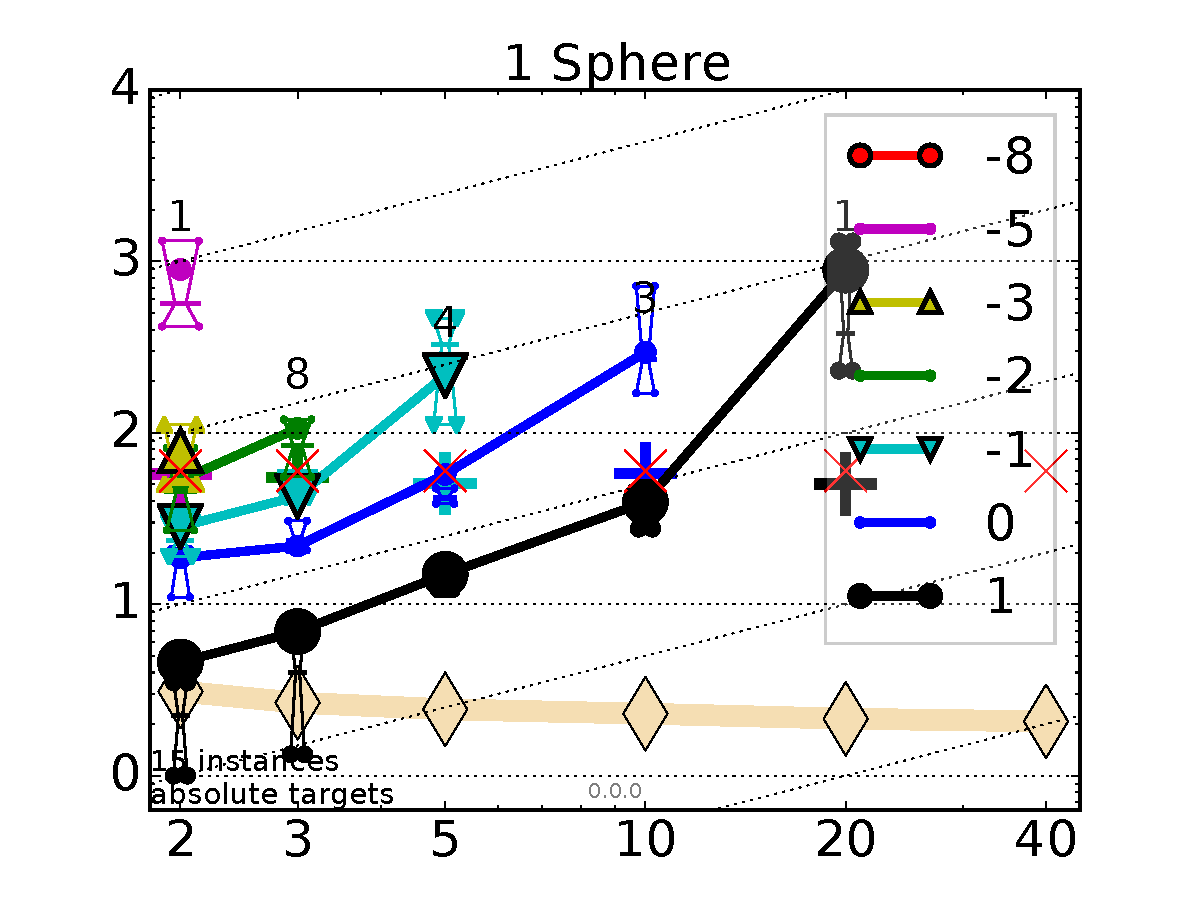
\includegraphics[width=0.268\textwidth]{ppfigdim_f001}&
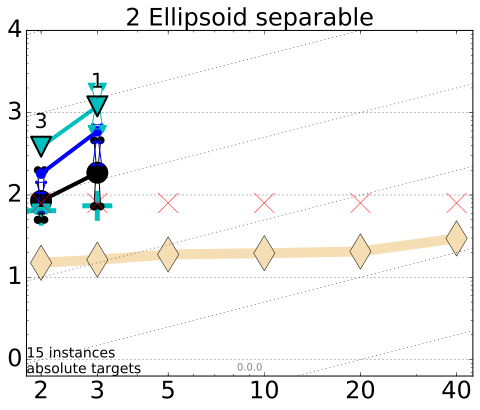
\includegraphics[width=0.268\textwidth]{ppfigdim_f002}&
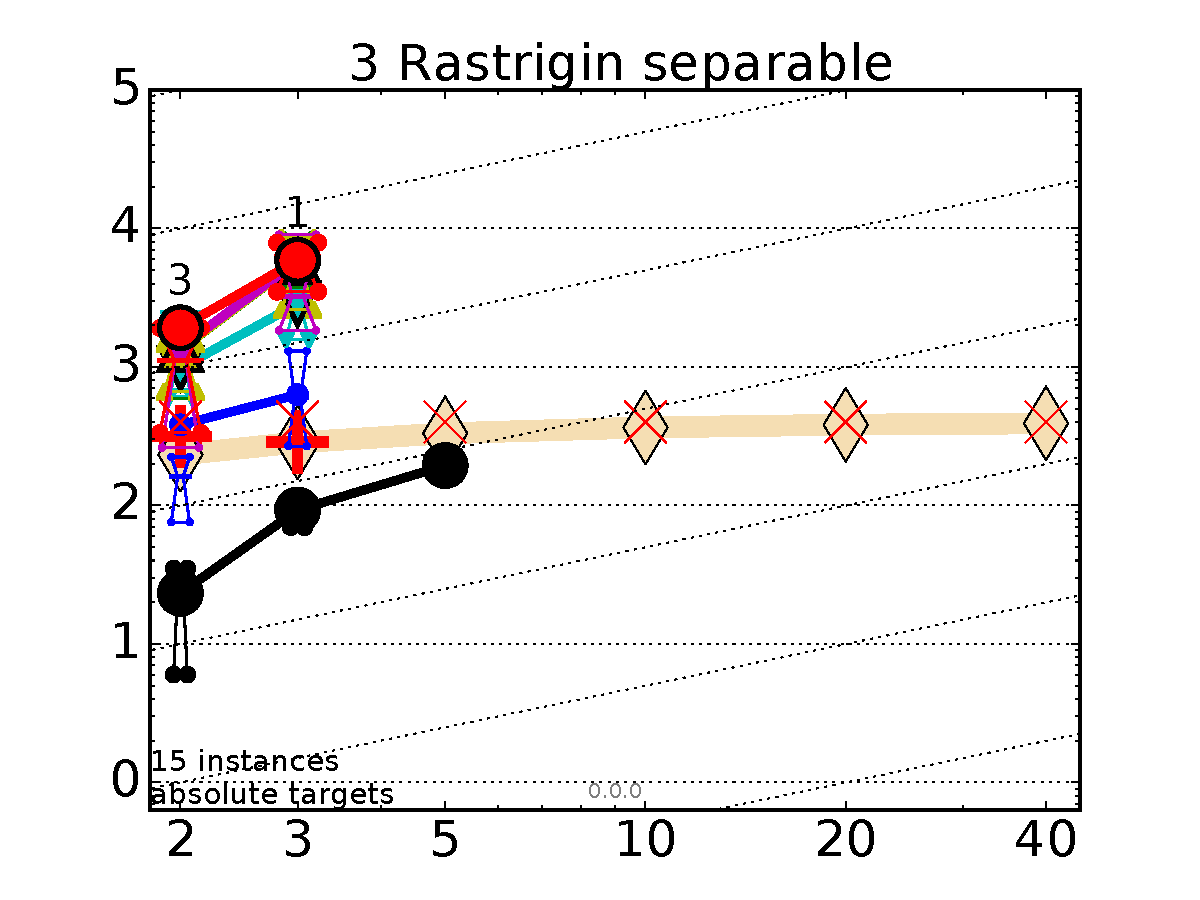
\includegraphics[width=0.268\textwidth]{ppfigdim_f003}&
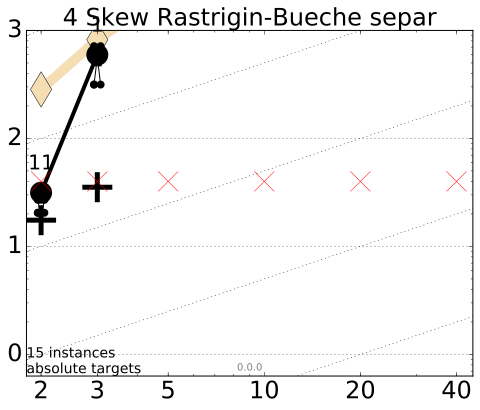
\includegraphics[width=0.268\textwidth]{ppfigdim_f004}\\[-2.2ex]
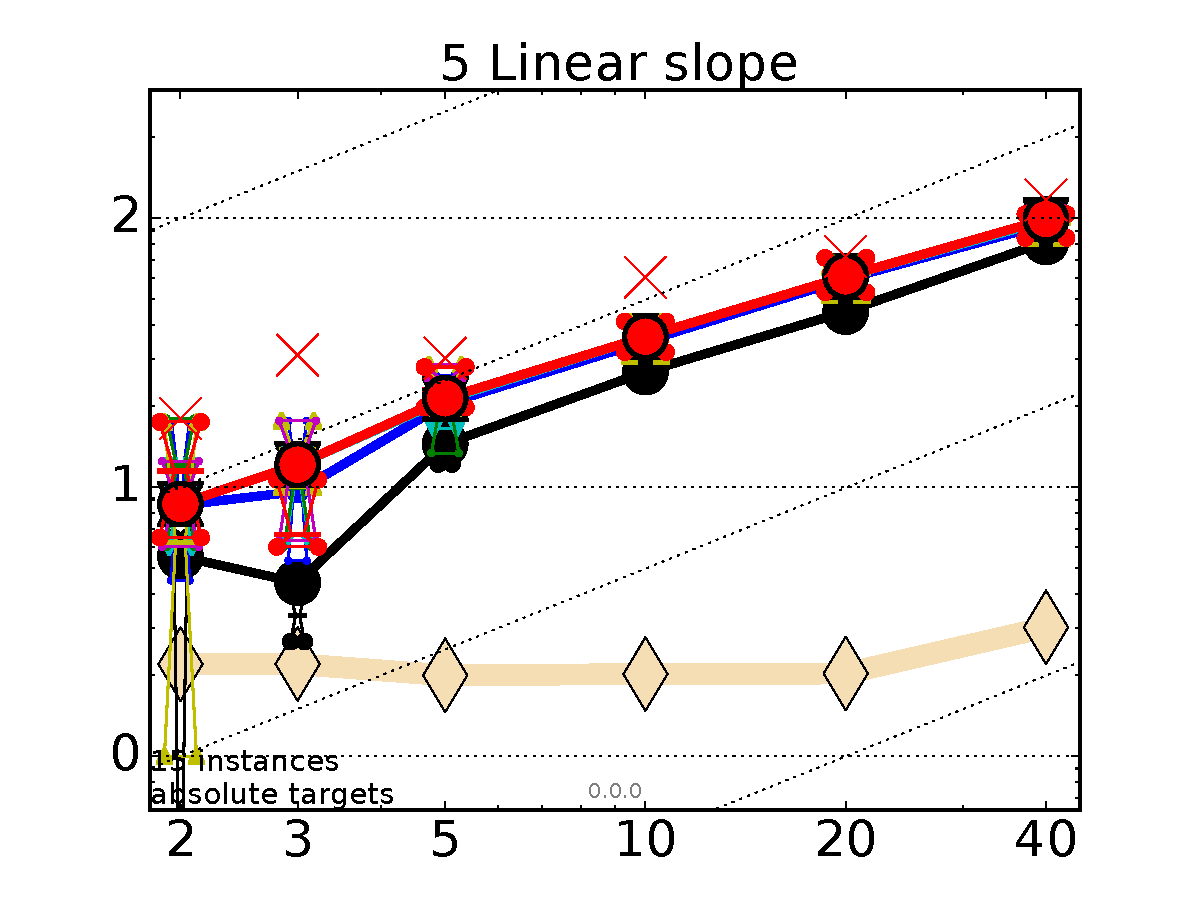
\includegraphics[width=0.268\textwidth]{ppfigdim_f005}&
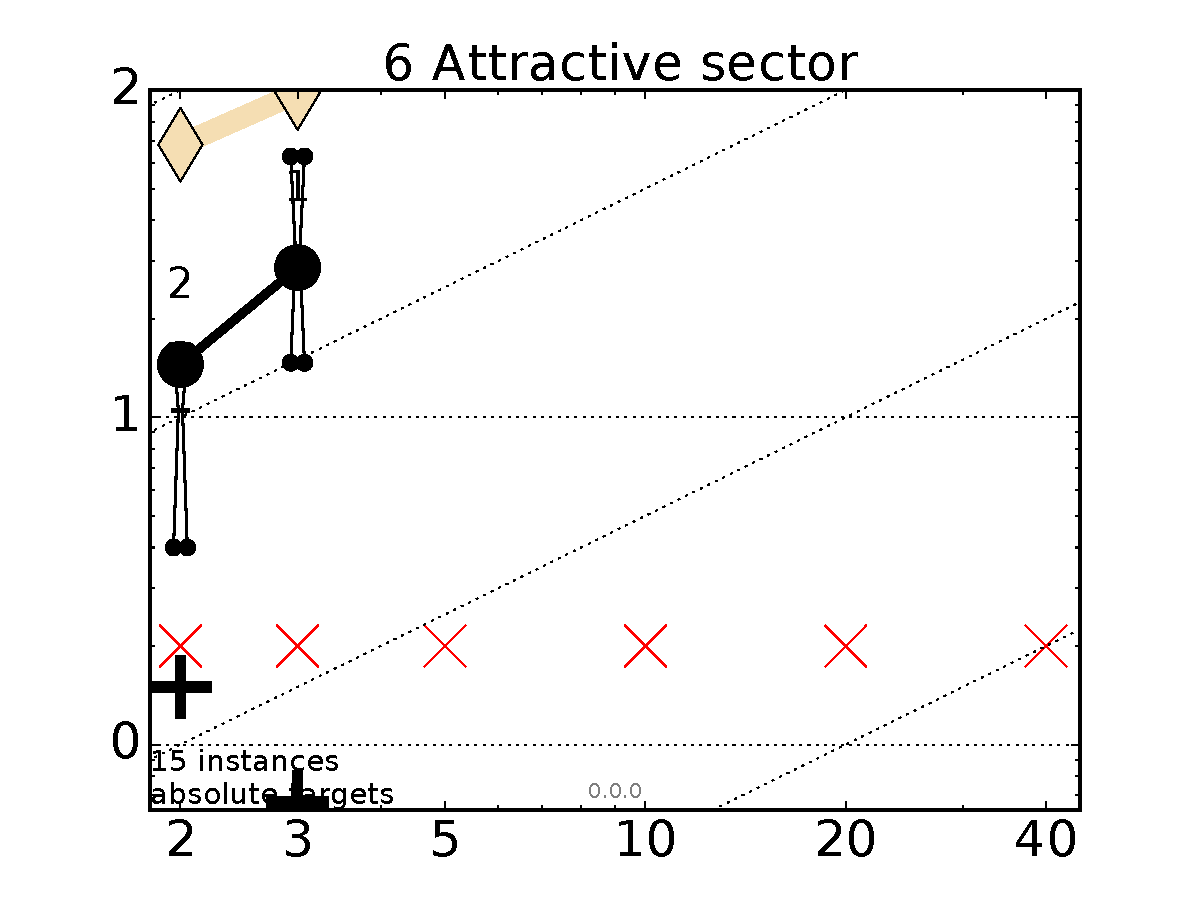
\includegraphics[width=0.268\textwidth]{ppfigdim_f006}&
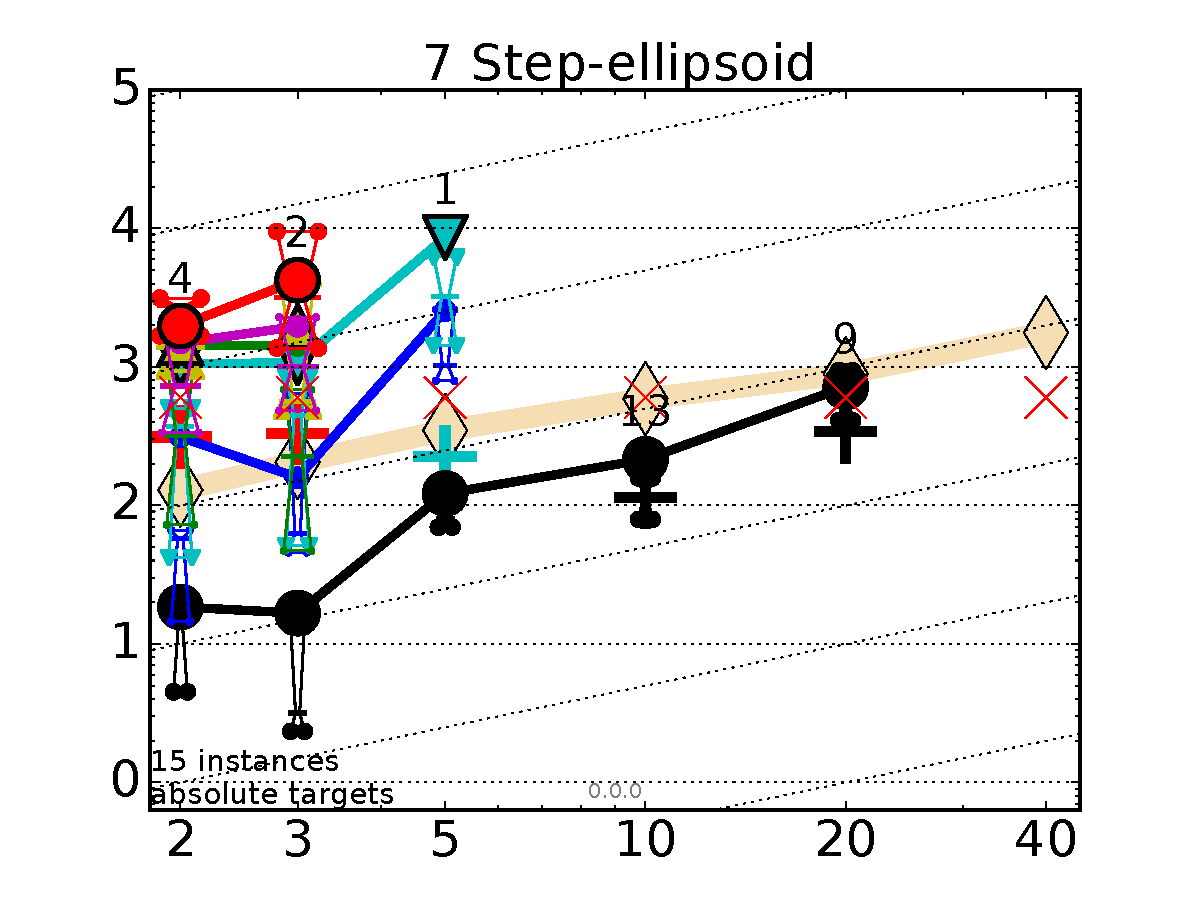
\includegraphics[width=0.268\textwidth]{ppfigdim_f007}&
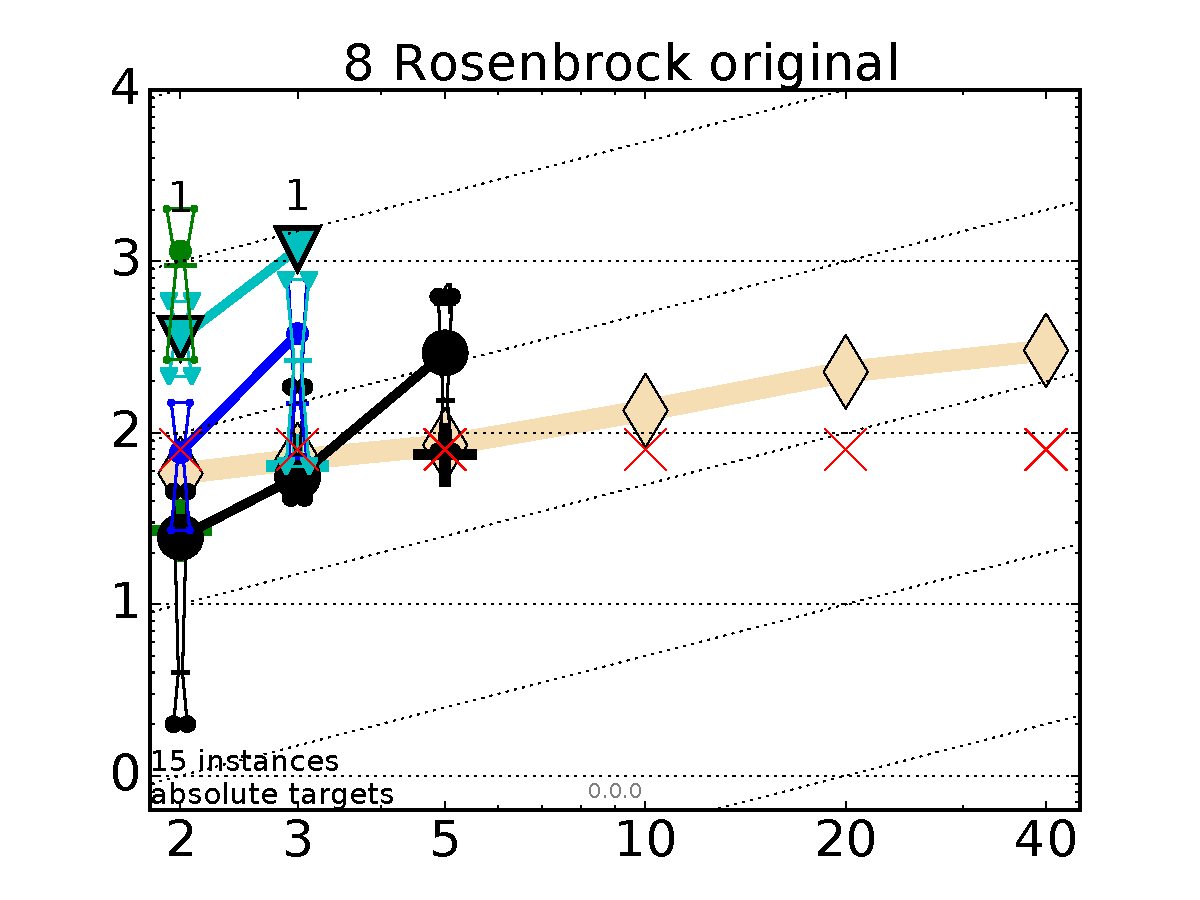
\includegraphics[width=0.268\textwidth]{ppfigdim_f008}\\[-2.2ex]
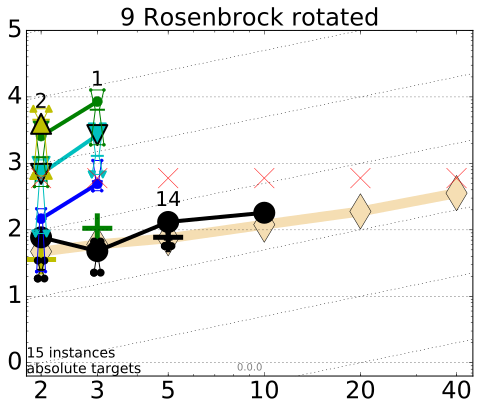
\includegraphics[width=0.268\textwidth]{ppfigdim_f009}&
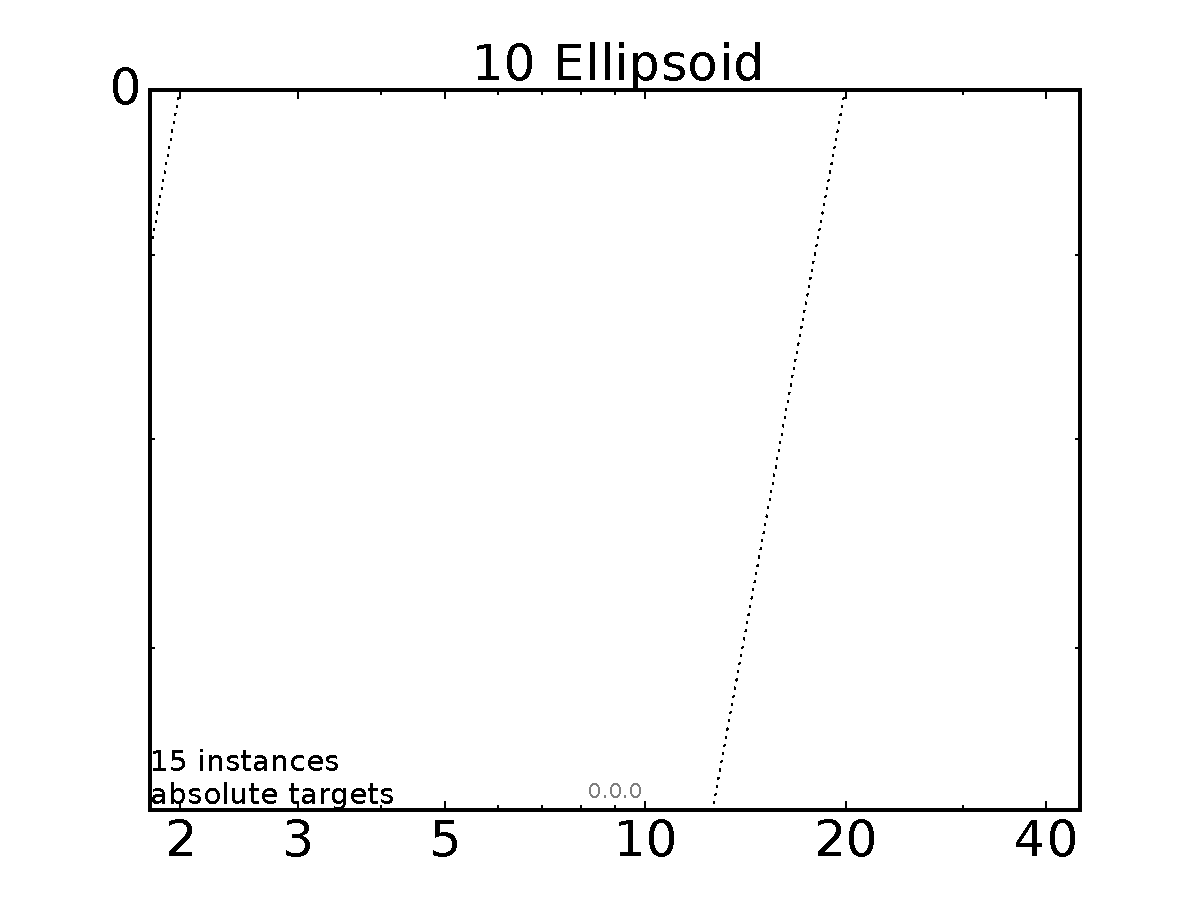
\includegraphics[width=0.268\textwidth]{ppfigdim_f010}&
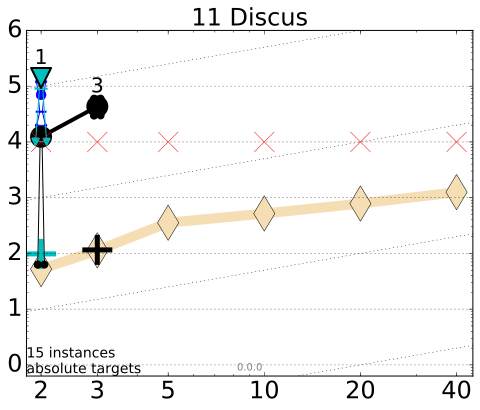
\includegraphics[width=0.268\textwidth]{ppfigdim_f011}&
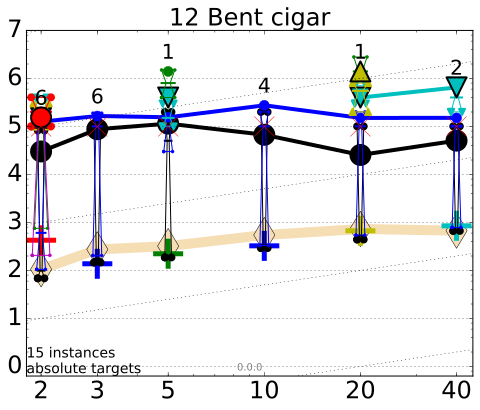
\includegraphics[width=0.268\textwidth]{ppfigdim_f012}\\[-2.2ex]
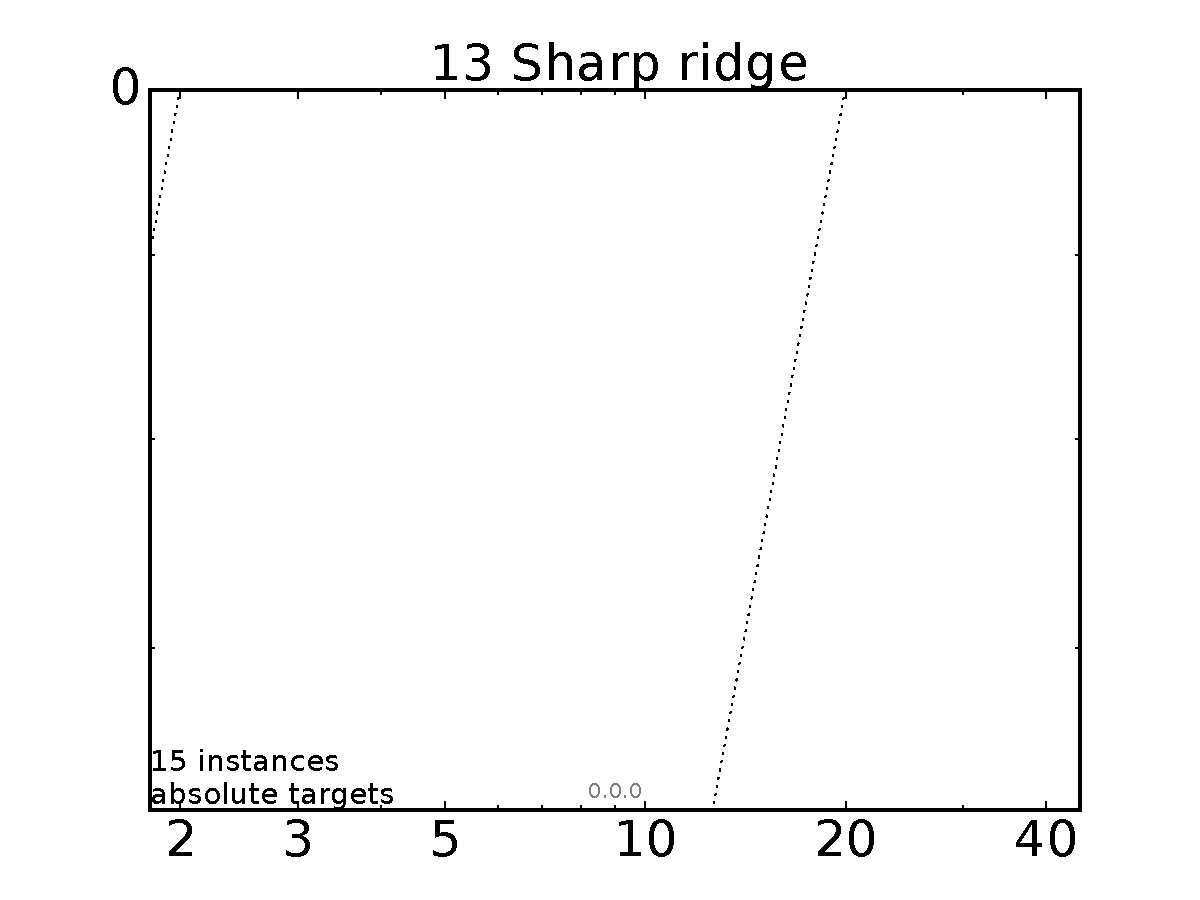
\includegraphics[width=0.268\textwidth]{ppfigdim_f013}&
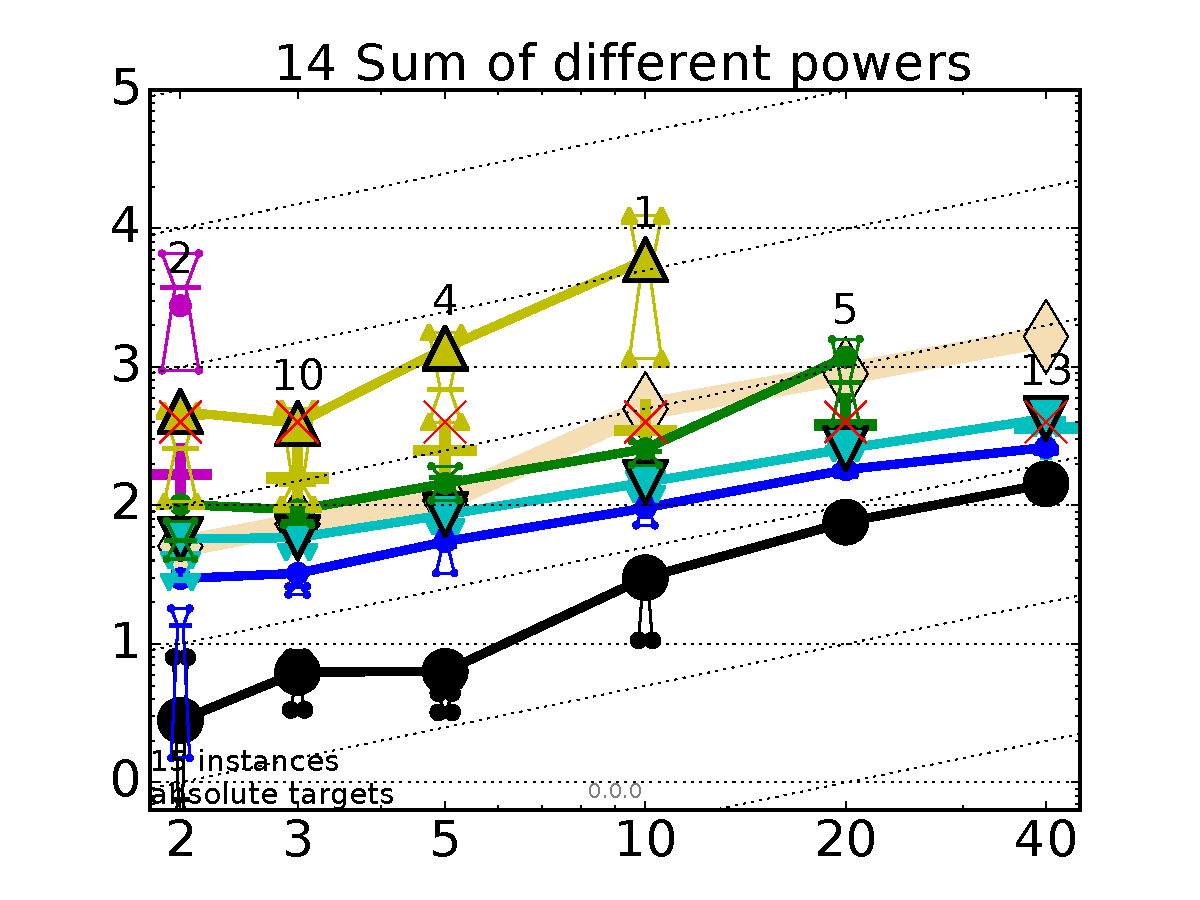
\includegraphics[width=0.268\textwidth]{ppfigdim_f014}&
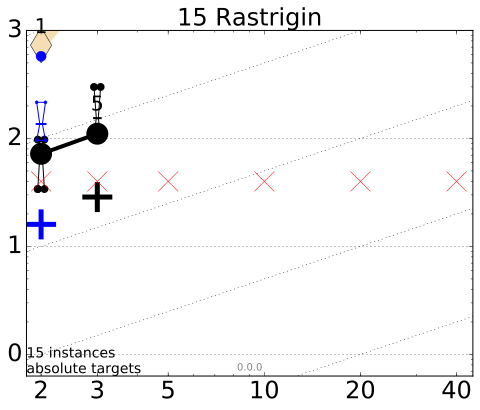
\includegraphics[width=0.268\textwidth]{ppfigdim_f015}&
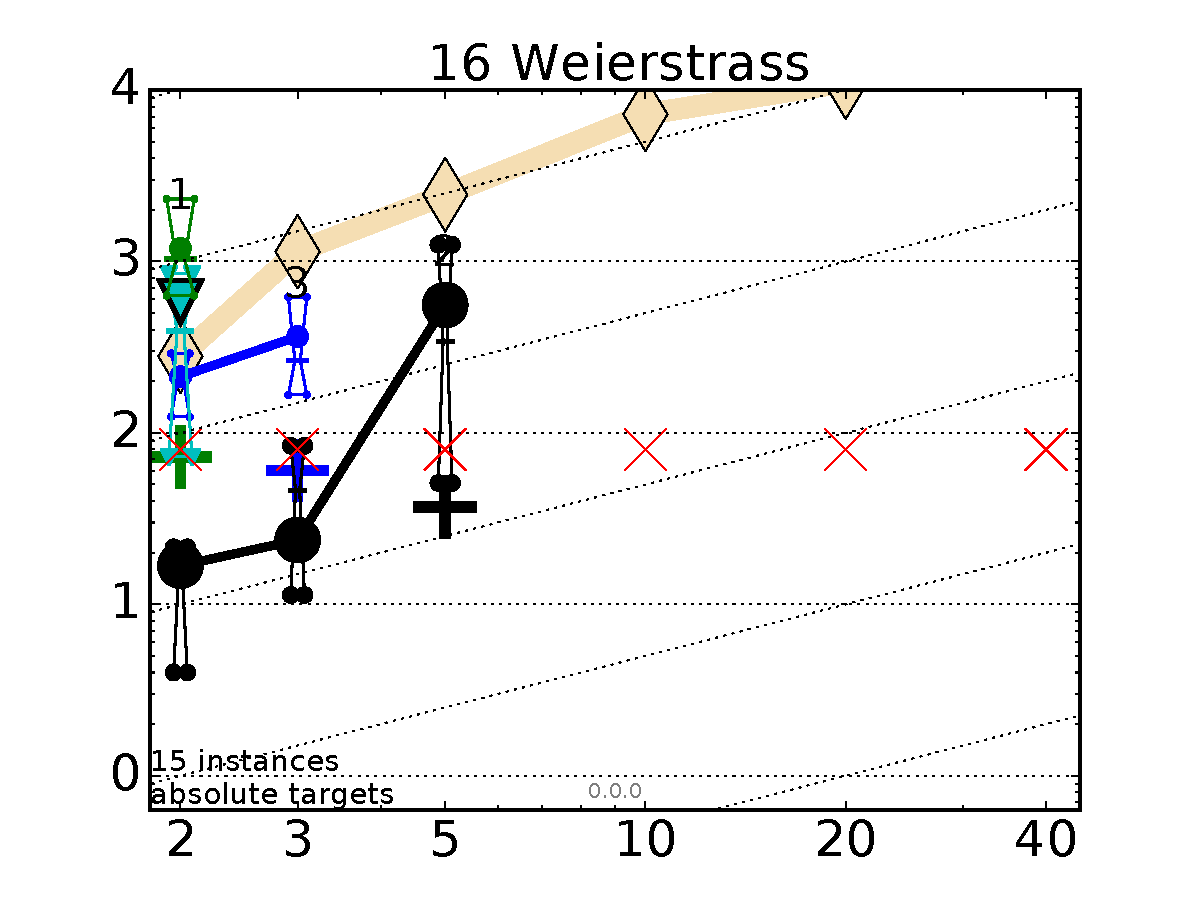
\includegraphics[width=0.268\textwidth]{ppfigdim_f016}\\[-2.2ex]
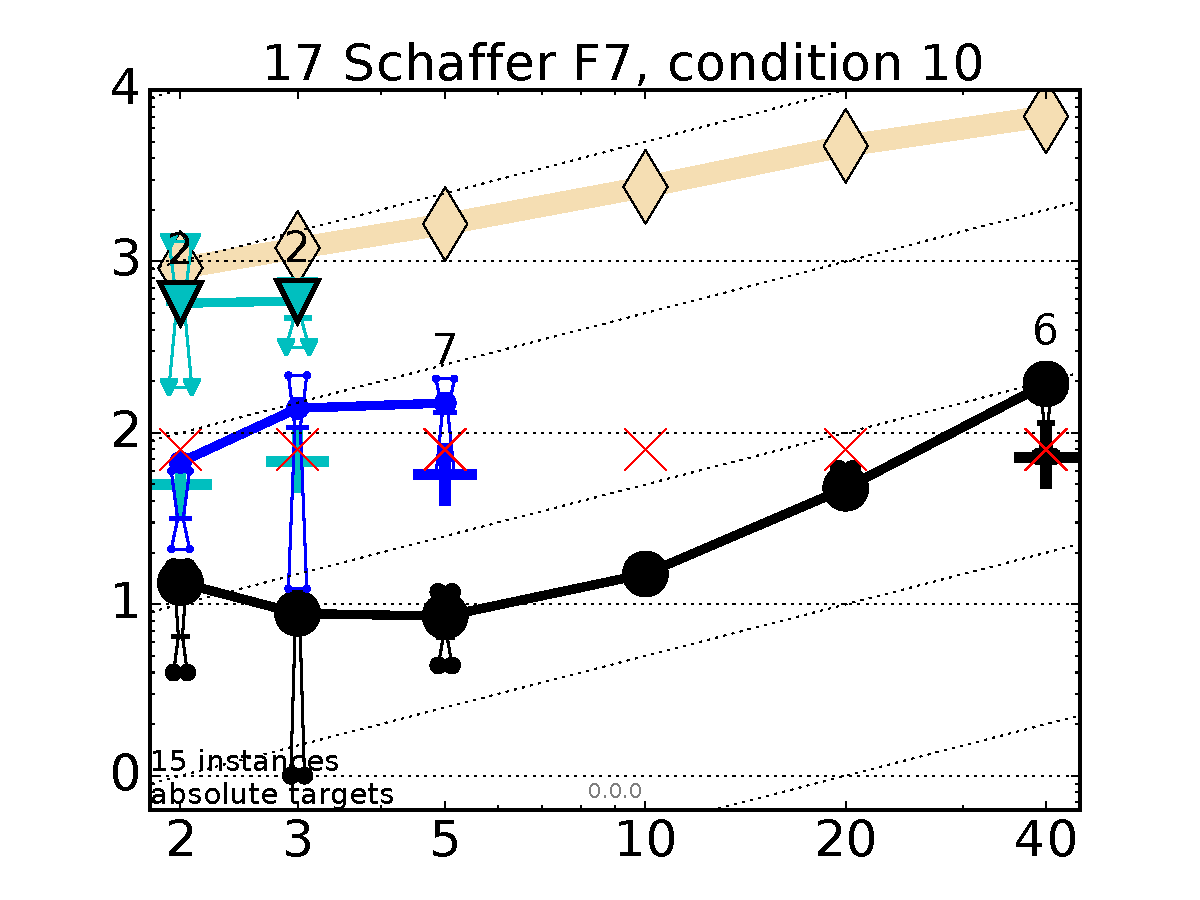
\includegraphics[width=0.268\textwidth]{ppfigdim_f017}&
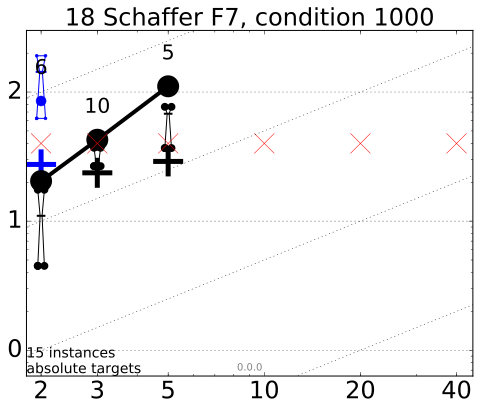
\includegraphics[width=0.268\textwidth]{ppfigdim_f018}&
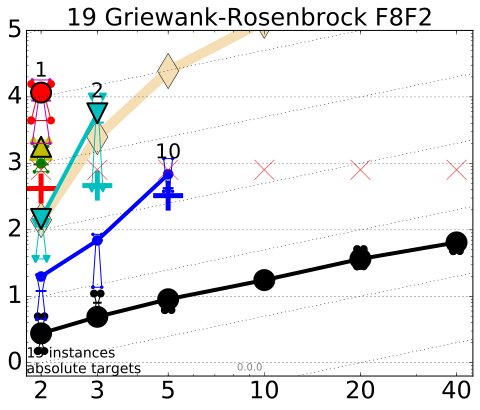
\includegraphics[width=0.268\textwidth]{ppfigdim_f019}&
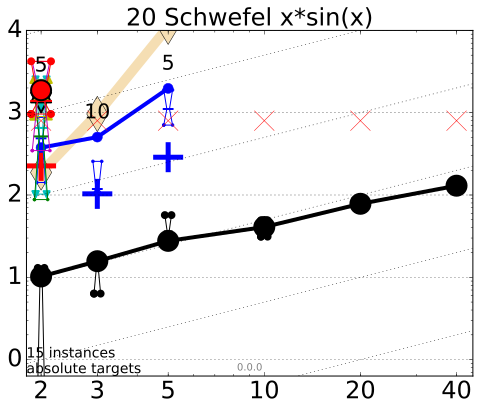
\includegraphics[width=0.268\textwidth]{ppfigdim_f020}\\[-2.2ex]
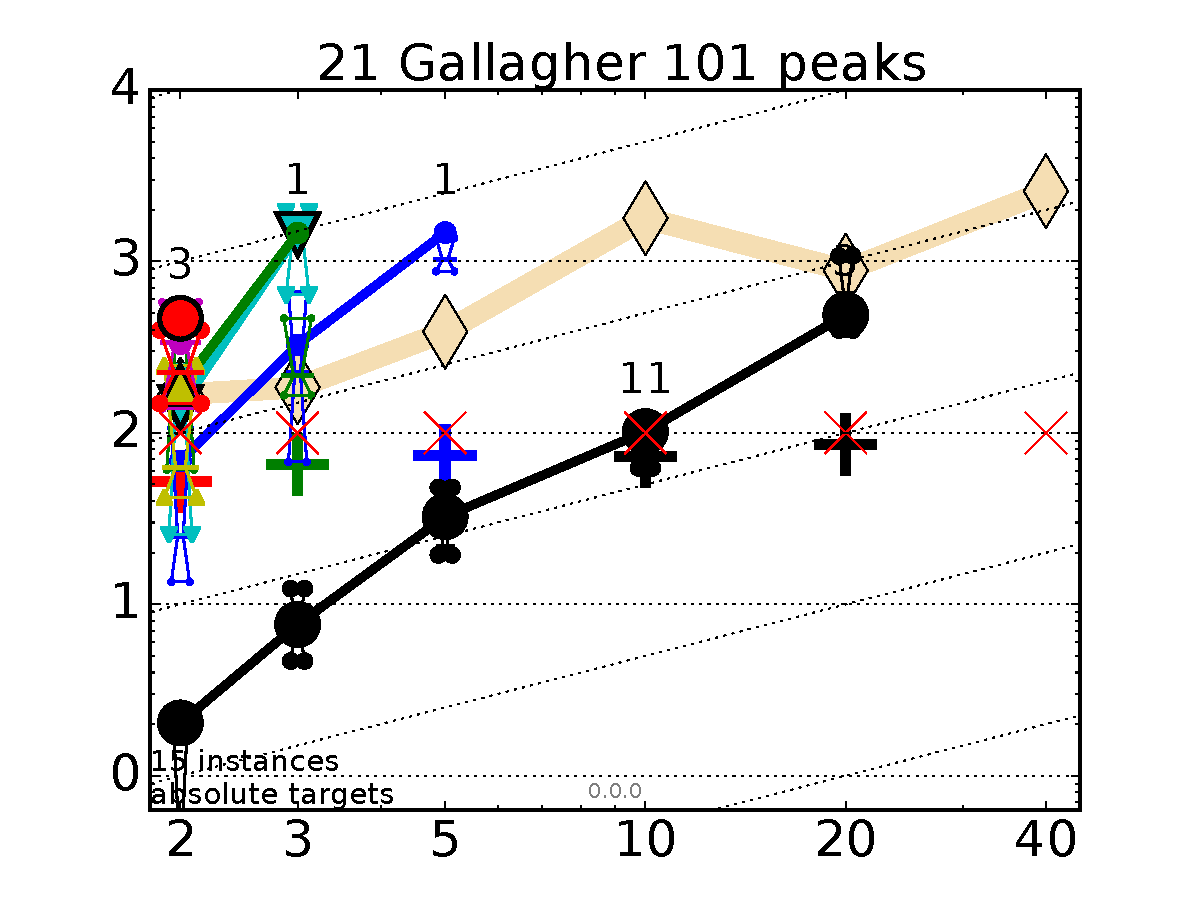
\includegraphics[width=0.268\textwidth]{ppfigdim_f021}&
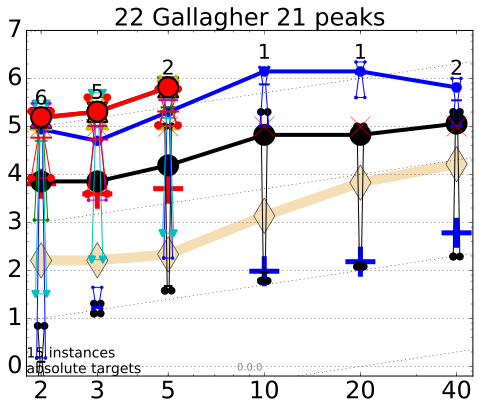
\includegraphics[width=0.268\textwidth]{ppfigdim_f022}&
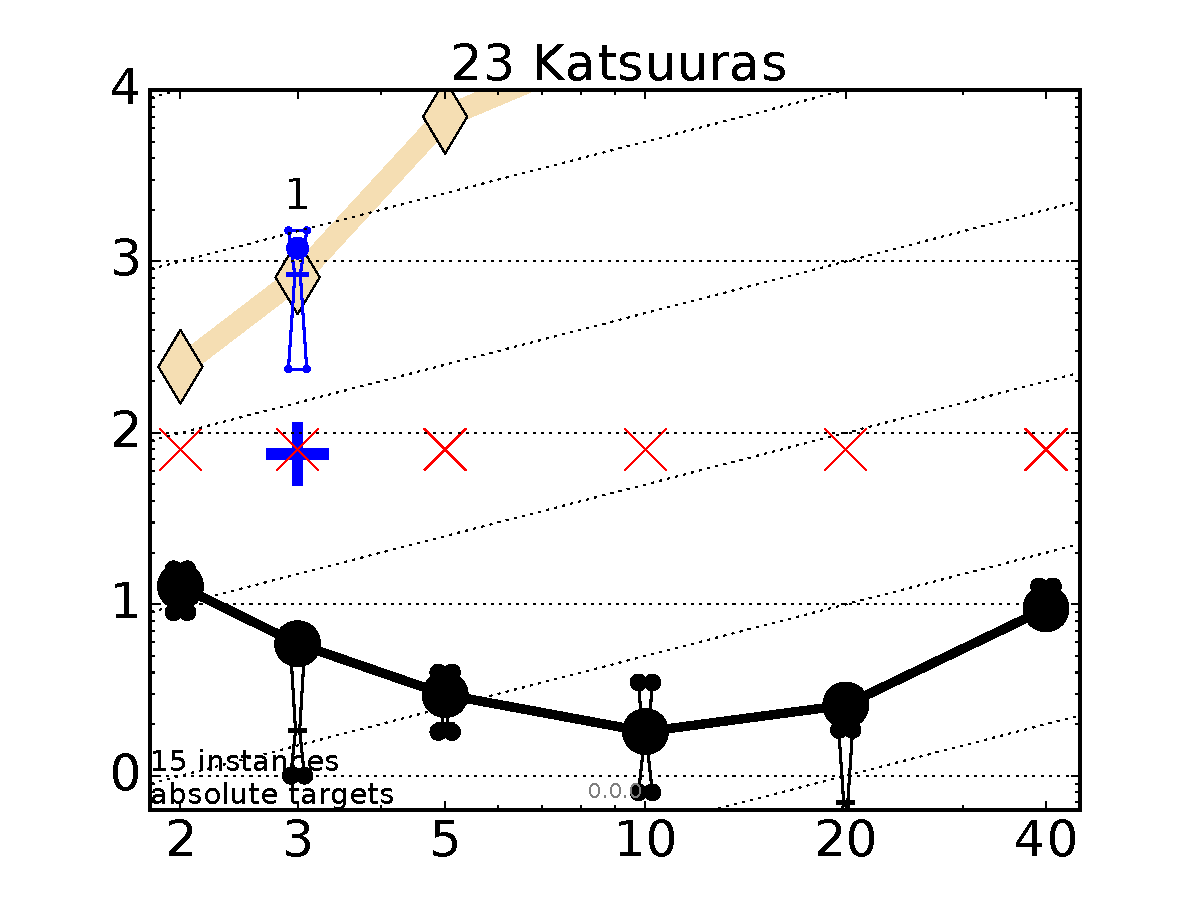
\includegraphics[width=0.268\textwidth]{ppfigdim_f023}&
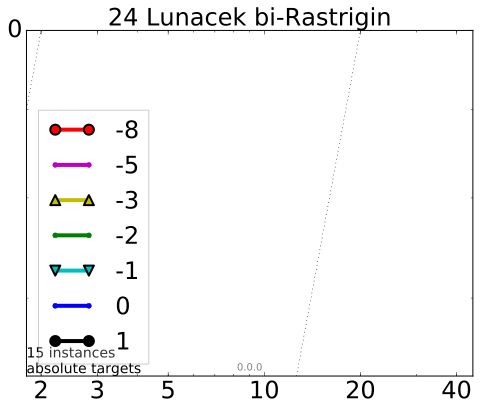
\includegraphics[width=0.268\textwidth]{ppfigdim_f024}
\end{tabular}
\vspace{-3ex}
 \caption{\label{fig:aRTgraphs}
 \bbobppfigdimlegend{$f_1$ and $f_{24}$}
 }
\end{figure*}

%%%%%%%%%%%%%%%%%%%%%%%%%%%%%%%%%%%%%%%%%%%%%%%%%%%%%%%%%%%%%%%%%%%%%%%%%%%%%%%
%%%%%%%%%%%%%%%%%%%%%%%%%%%%%%%%%%%%%%%%%%%%%%%%%%%%%%%%%%%%%%%%%%%%%%%%%%%%%%%
 
% Table showing the average runtime (aRT in number of function
% evaluations) divided by the best aRT measured during BBOB-2009 (given in the
% first row of each cell) for functions $f_1$--$f_{24}$.

%%%%%%%%%%%%%%%%%%%%%%%%%%%%%%%%%%%%%%%%%%%%%%%%%%%%%%%%%%%%%%%%%%%%%%%%%%%%%%%

\begin{table*}
\centering {\tiny
\parbox{0.499\textwidth}{\centering
   {\small 5-D}\\
   \input{\bbobdatapath\algfolder pptable_05D_noiselessall}}%
\parbox{0.499\textwidth}{\centering
   {\small 20-D}\\
   \input{\bbobdatapath\algfolder pptable_20D_noiselessall}}}%
\caption[Table of aRTs]{\label{tab:aRTs}\bbobpptablecaption{} 
}
\end{table*}
%%%%%%%%%%%%%%%%%%%%%%%%%%%%%%%%%%%%%%%%%%%%%%%%%%%%%%%%%%%%%%%%%%%%%%%%%%%%%%%
%%%%%%%%%%%%%%%%%%%%%%%%%%%%%%%%%%%%%%%%%%%%%%%%%%%%%%%%%%%%%%%%%%%%%%%%%%%%%%%


%%%%%%%%%%%%%%%%%%%%%%%%%%%%%%%%%%%%%%%%%%%%%%%%%%%%%%%%%%%%%%%%%%%%%%%%%%%%%%%
%%%%%%%%%%%%%%%%%%%%%%%%%%%%%%%%%%%%%%%%%%%%%%%%%%%%%%%%%%%%%%%%%%%%%%%%%%%%%%%

% Empirical cumulative distribution functions (ECDFs) per function group.

%%%%%%%%%%%%%%%%%%%%%%%%%%%%%%%%%%%%%%%%%%%%%%%%%%%%%%%%%%%%%%%%%%%%%%%%%%%%%%%
\newcommand{\rot}[2][2.5]{
  \hspace*{-3.5\baselineskip}%
  \begin{rotate}{90}\hspace{#1em}#2
  \end{rotate}}
\begin{figure*}
\begin{tabular}{l@{\hspace*{-0.025\textwidth}}l@{\hspace*{-0.00\textwidth}}|l@{\hspace*{-0.025\textwidth}}l}
\multicolumn{2}{c}{$D=5$} & \multicolumn{2}{c}{$D=20$}\\[-0.5ex]
\rot{separable fcts}
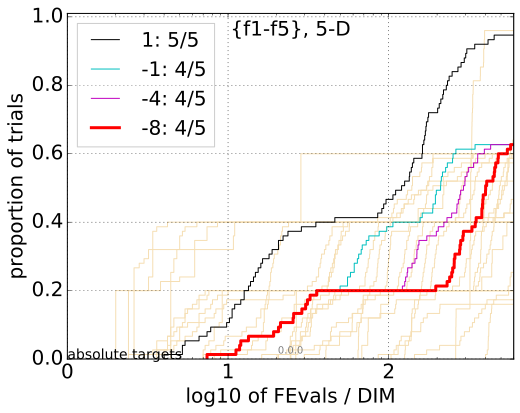
\includegraphics[width=0.268\textwidth,trim=0 0 0 13mm, clip]{pprldistr_05D_separ} &
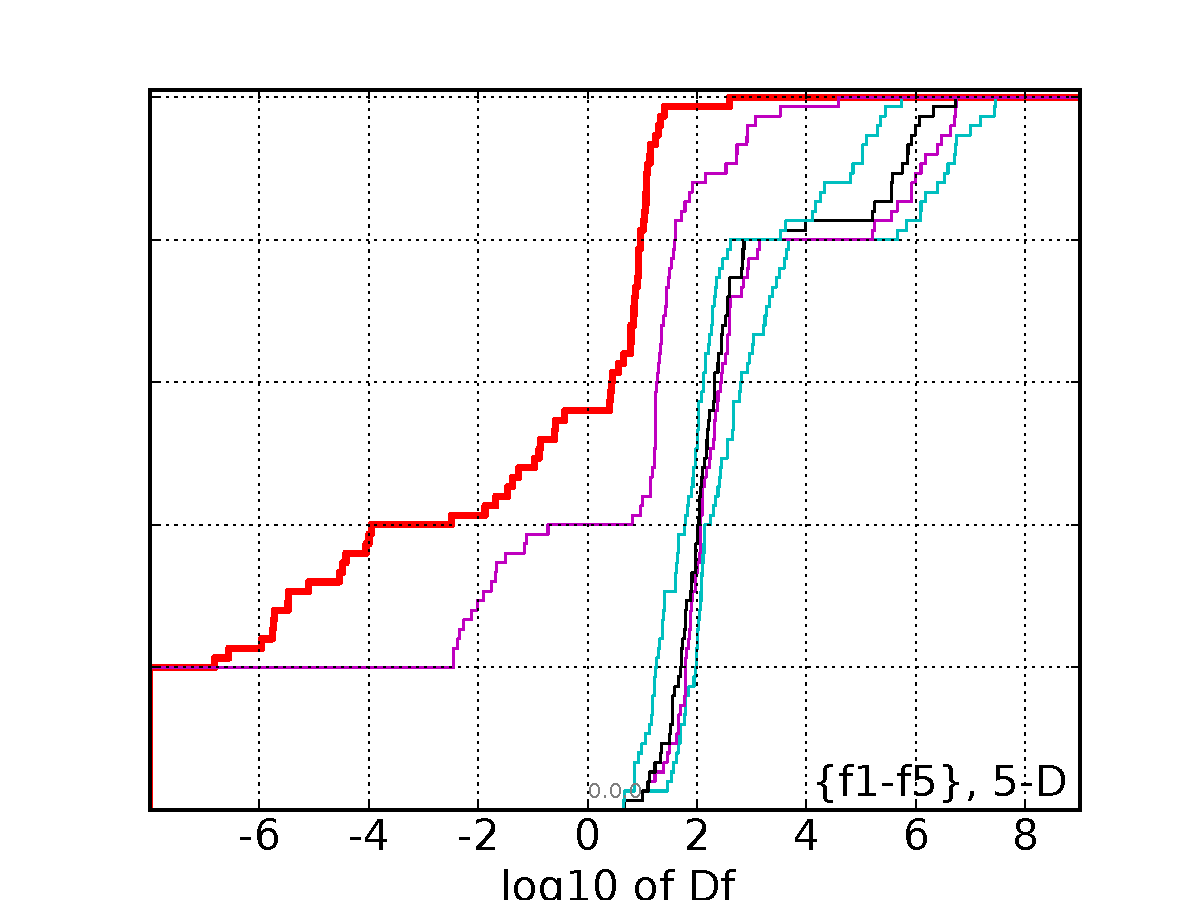
\includegraphics[width=0.2362\textwidth,trim=2.40cm 0 0 13mm, clip]{ppfvdistr_05D_separ} &
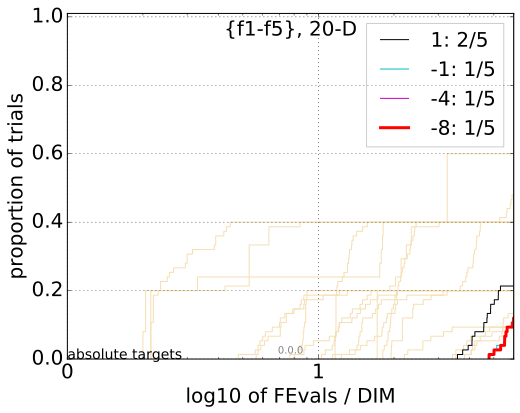
\includegraphics[width=0.268\textwidth,trim=0 0 0 13mm, clip]{pprldistr_20D_separ} &
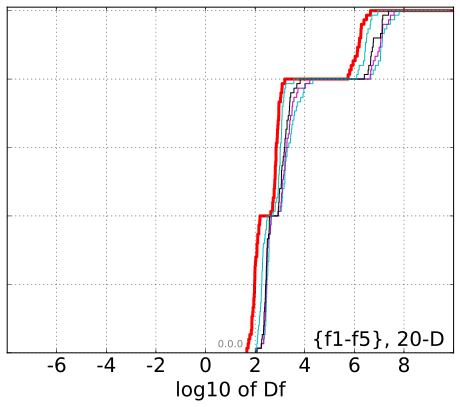
\includegraphics[width=0.2362\textwidth,trim=2.40cm 0 0 13mm, clip]{ppfvdistr_20D_separ} \\[-2ex]
\rot[1]{misc.\ moderate fcts}
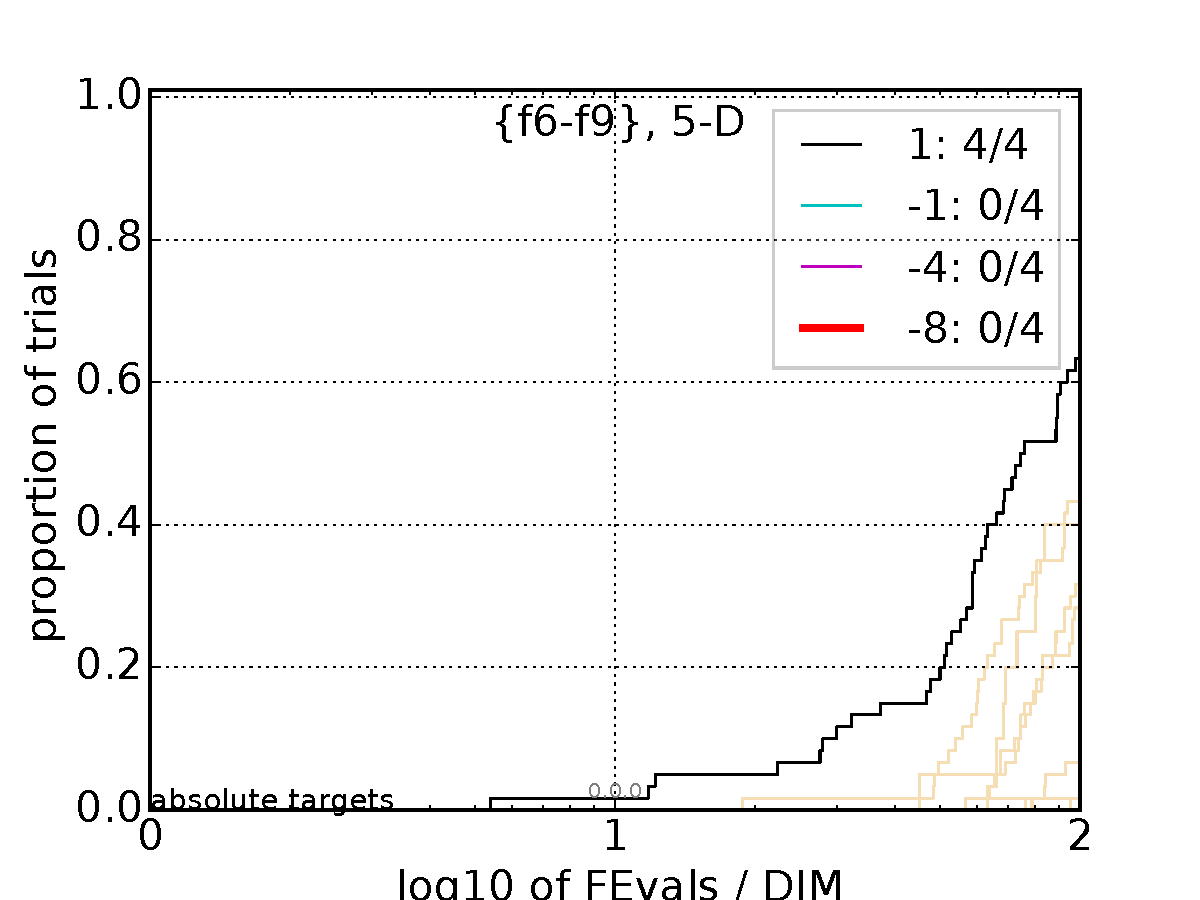
\includegraphics[width=0.268\textwidth,trim=0 0 0 13mm, clip]{pprldistr_05D_lcond} &
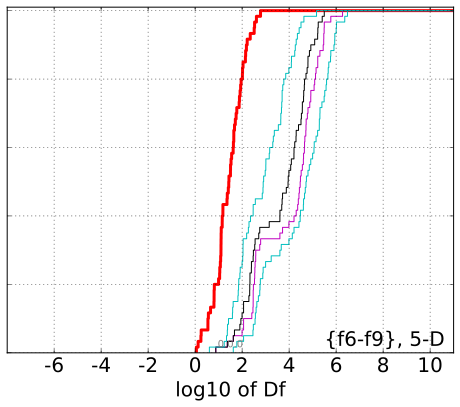
\includegraphics[width=0.2362\textwidth,trim=2.40cm 0 0 13mm, clip]{ppfvdistr_05D_lcond} &
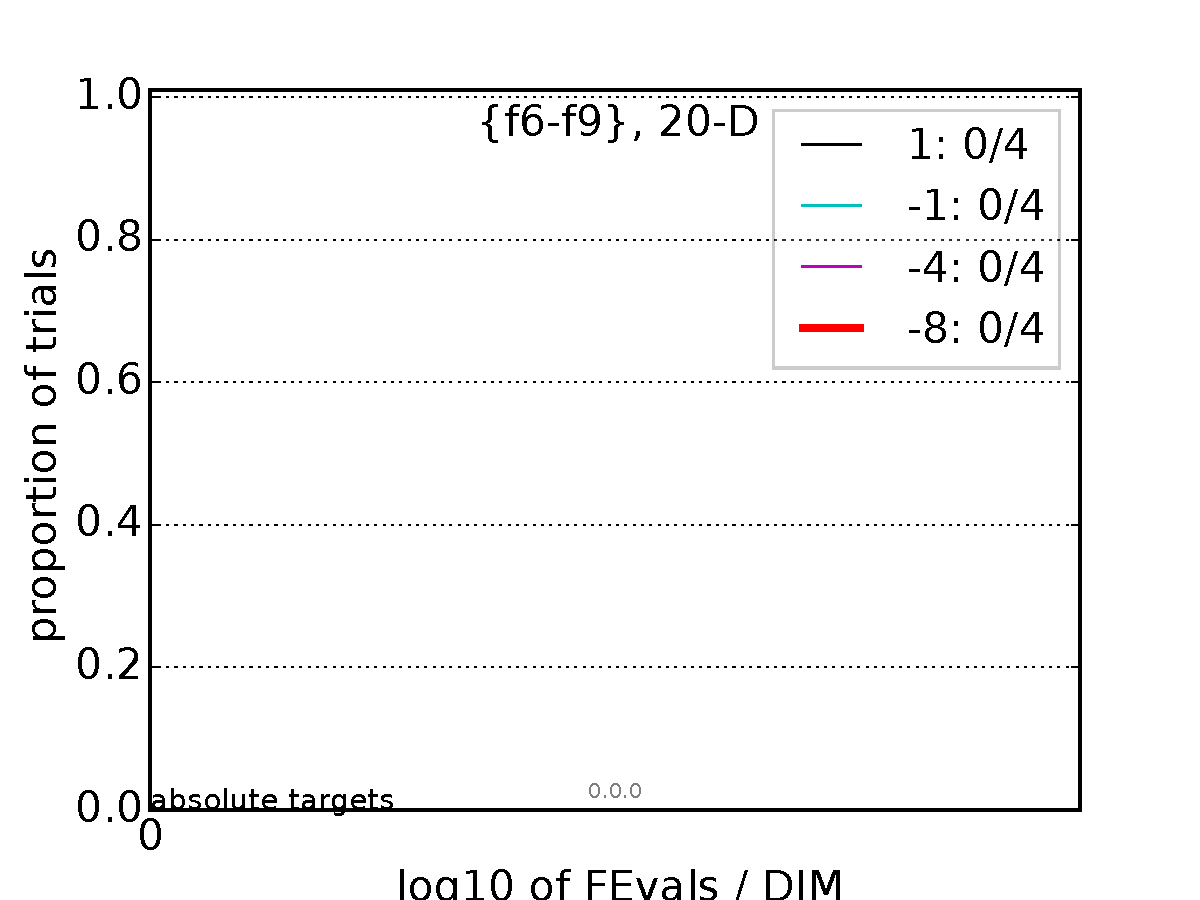
\includegraphics[width=0.268\textwidth,trim=0 0 0 13mm, clip]{pprldistr_20D_lcond} &
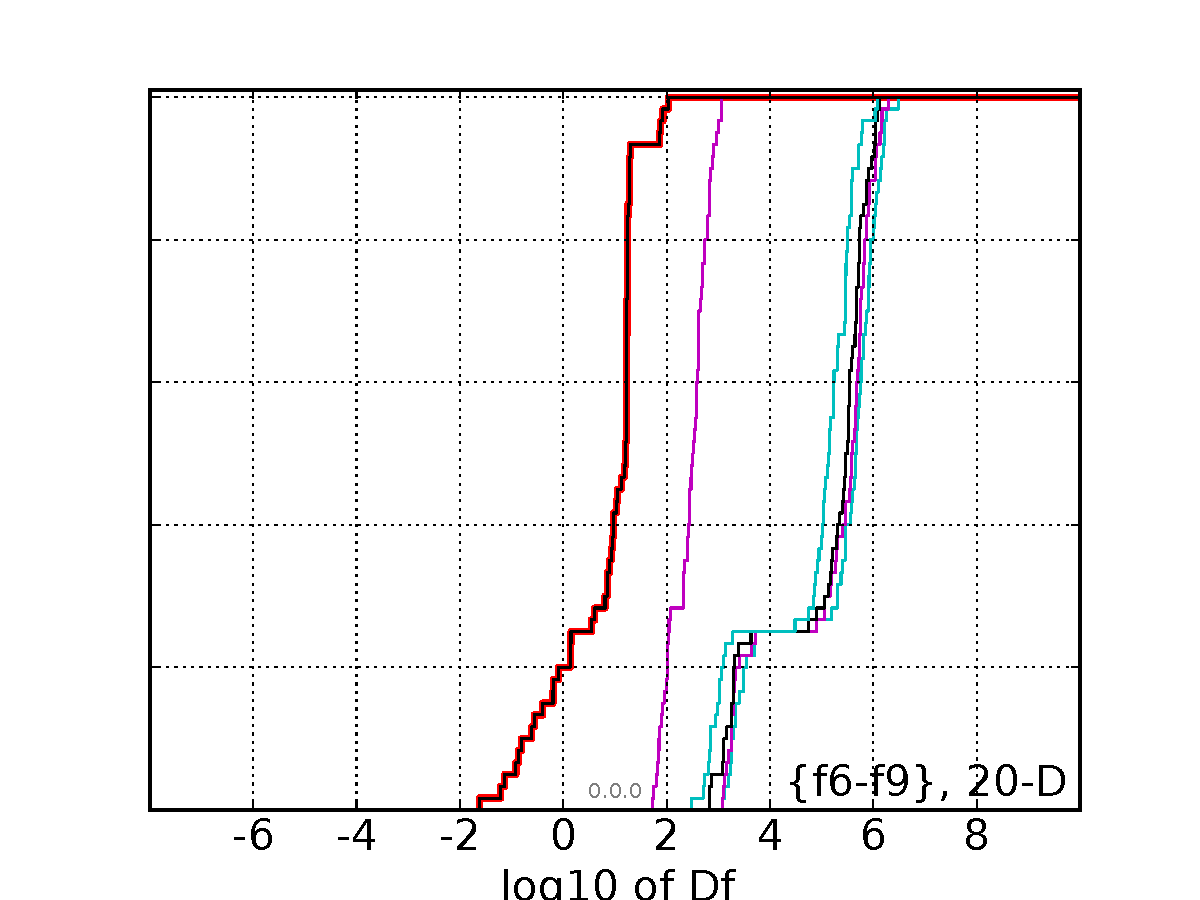
\includegraphics[width=0.2362\textwidth,trim=2.40cm 0 0 13mm, clip]{ppfvdistr_20D_lcond} \\[-2ex]
\rot[1.3]{ill-conditioned fcts}
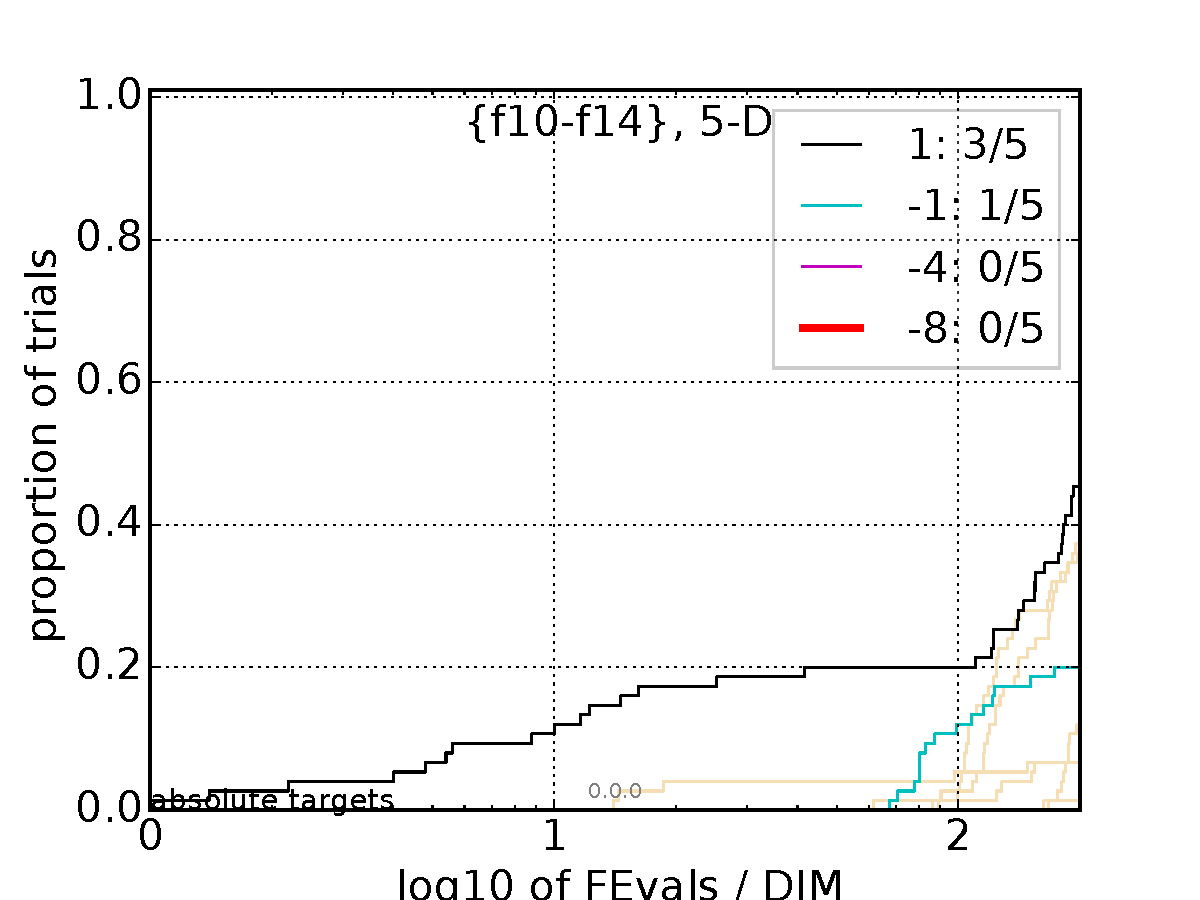
\includegraphics[width=0.268\textwidth,trim=0 0 0 13mm, clip]{pprldistr_05D_hcond} &
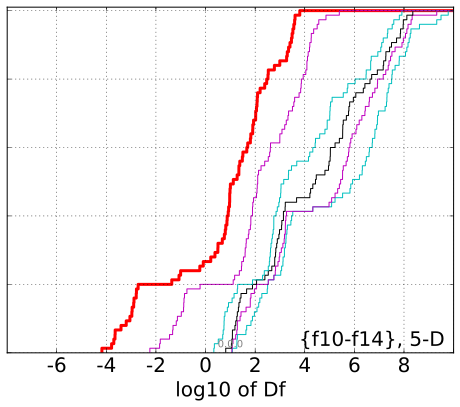
\includegraphics[width=0.2362\textwidth,trim=2.40cm 0 0 13mm, clip]{ppfvdistr_05D_hcond} &
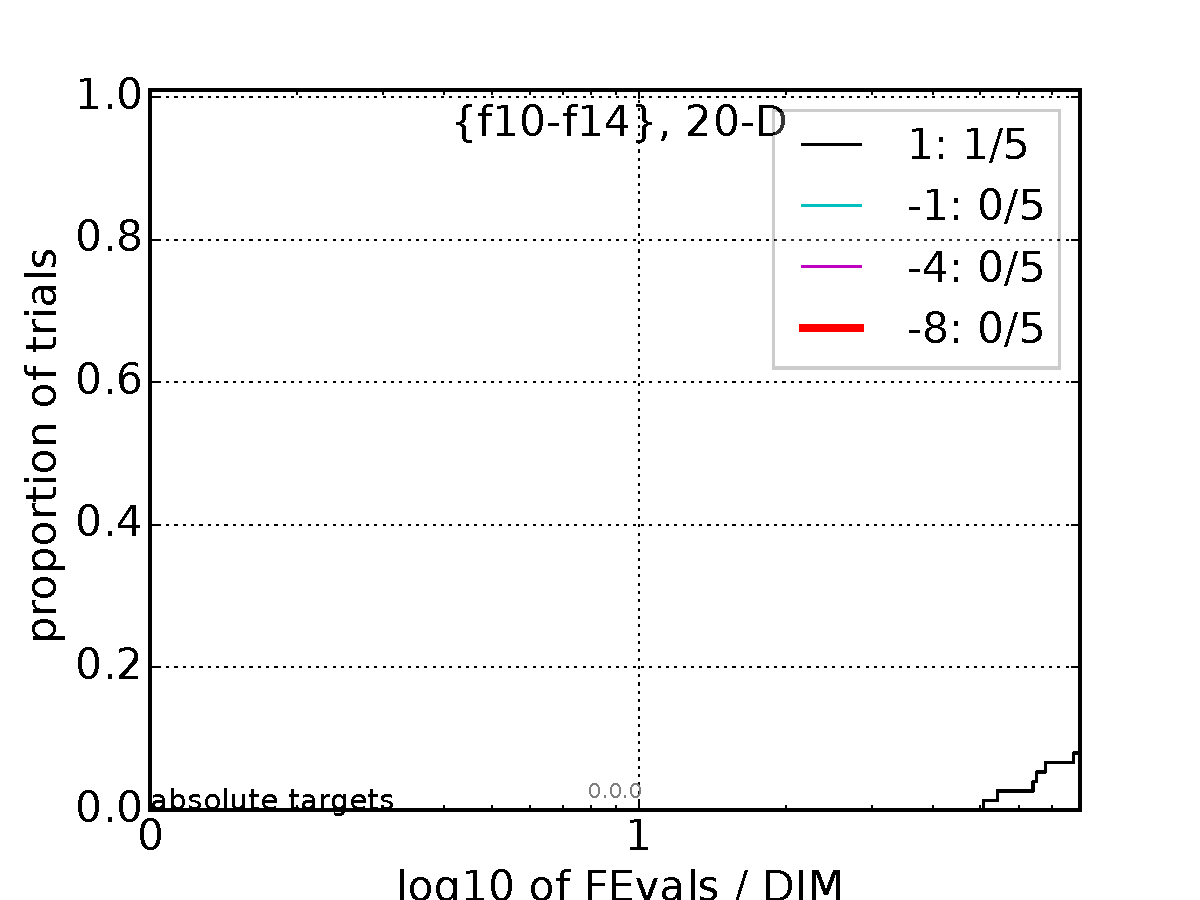
\includegraphics[width=0.268\textwidth,trim=0 0 0 13mm, clip]{pprldistr_20D_hcond} &
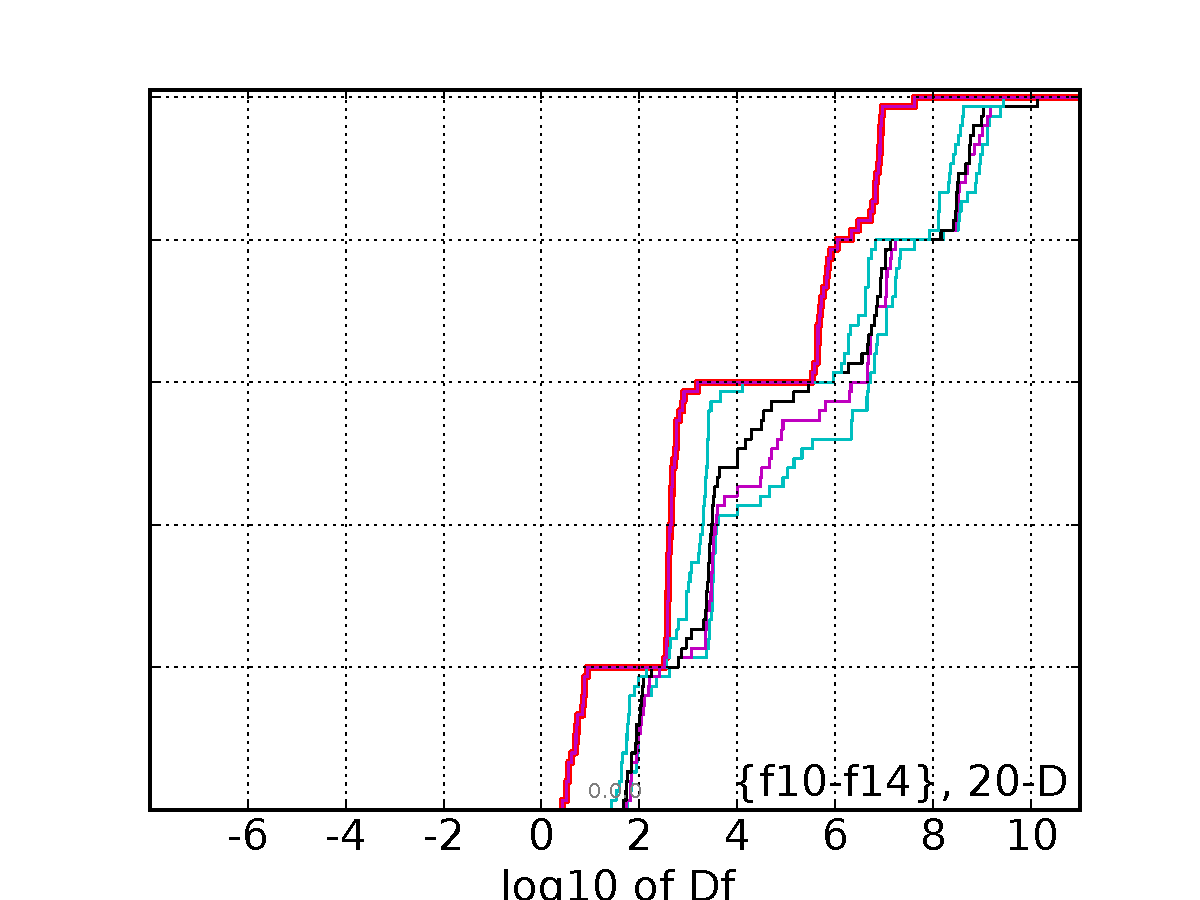
\includegraphics[width=0.2362\textwidth,trim=2.40cm 0 0 13mm, clip]{ppfvdistr_20D_hcond} \\[-2ex]
\rot[1.6]{multi-modal fcts}
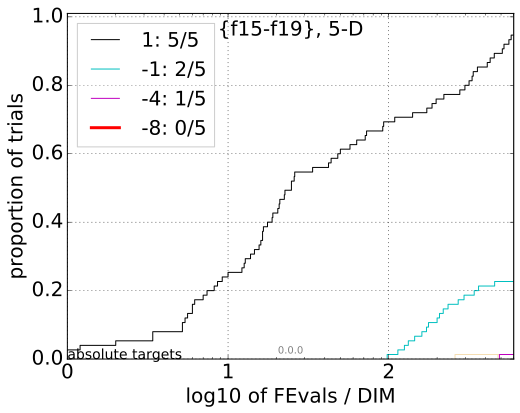
\includegraphics[width=0.268\textwidth,trim=0 0 0 13mm, clip]{pprldistr_05D_multi} &
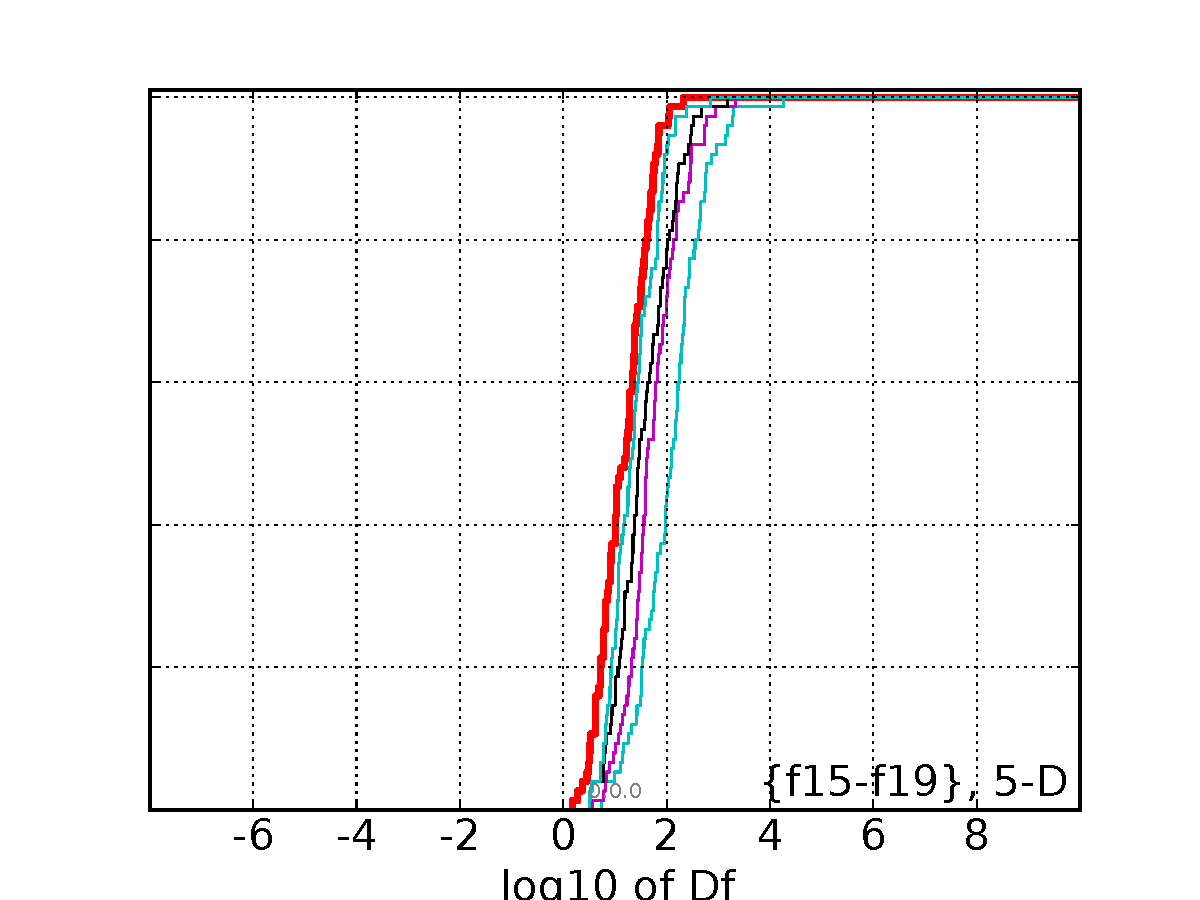
\includegraphics[width=0.2362\textwidth,trim=2.40cm 0 0 13mm, clip]{ppfvdistr_05D_multi} &
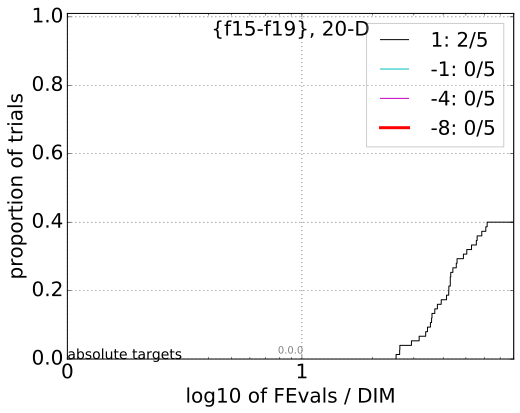
\includegraphics[width=0.268\textwidth,trim=0 0 0 13mm, clip]{pprldistr_20D_multi} &
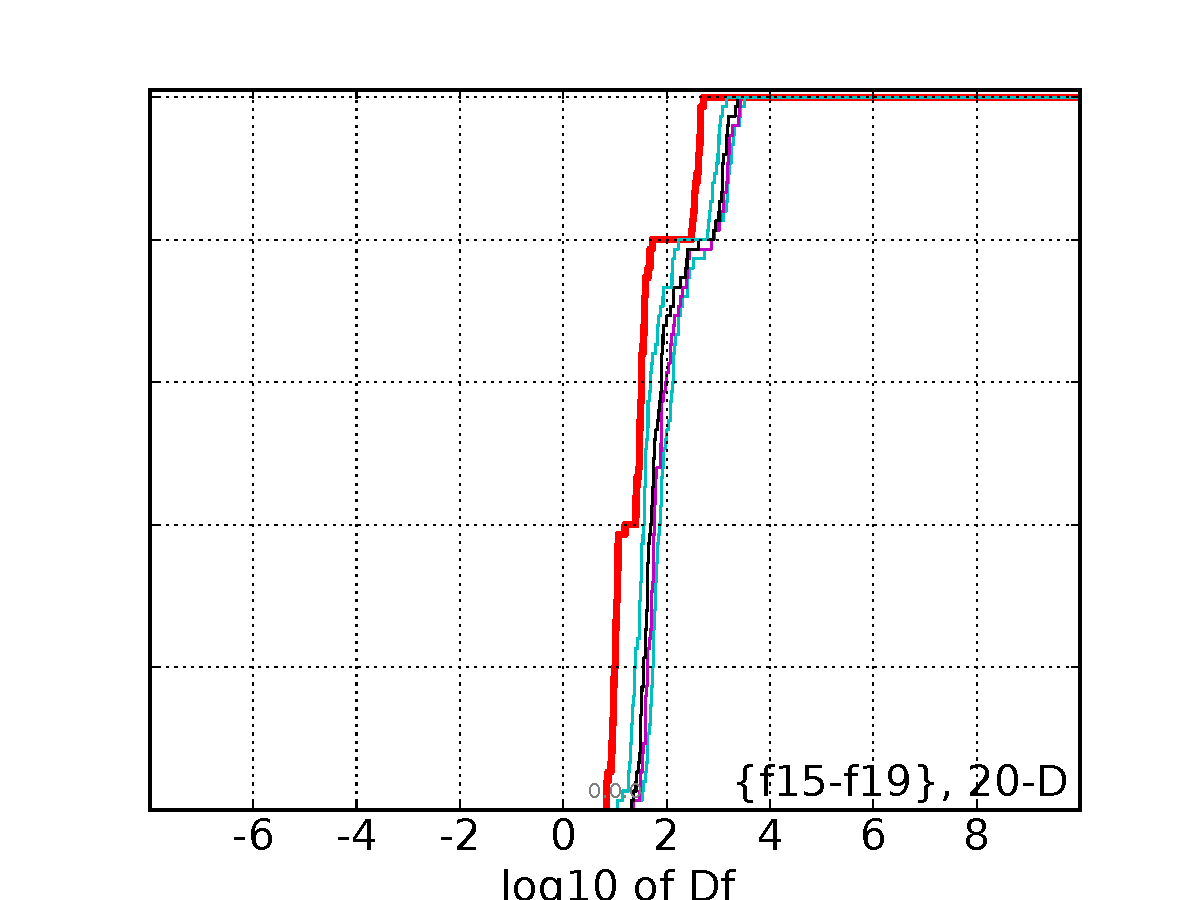
\includegraphics[width=0.2362\textwidth,trim=2.40cm 0 0 13mm, clip]{ppfvdistr_20D_multi} \\[-2ex]
\rot[1.0]{weak structure fcts}
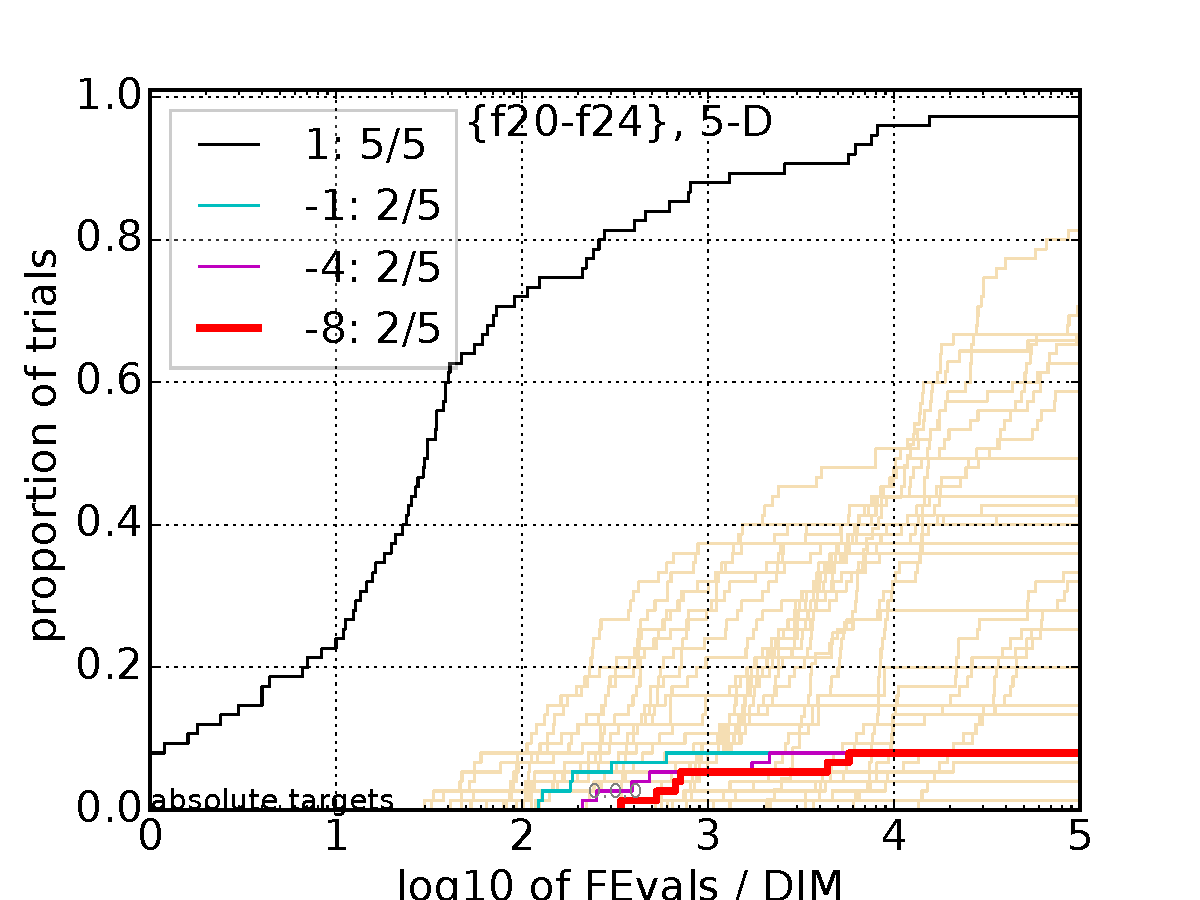
\includegraphics[width=0.268\textwidth,trim=0 0 0 13mm, clip]{pprldistr_05D_mult2} &
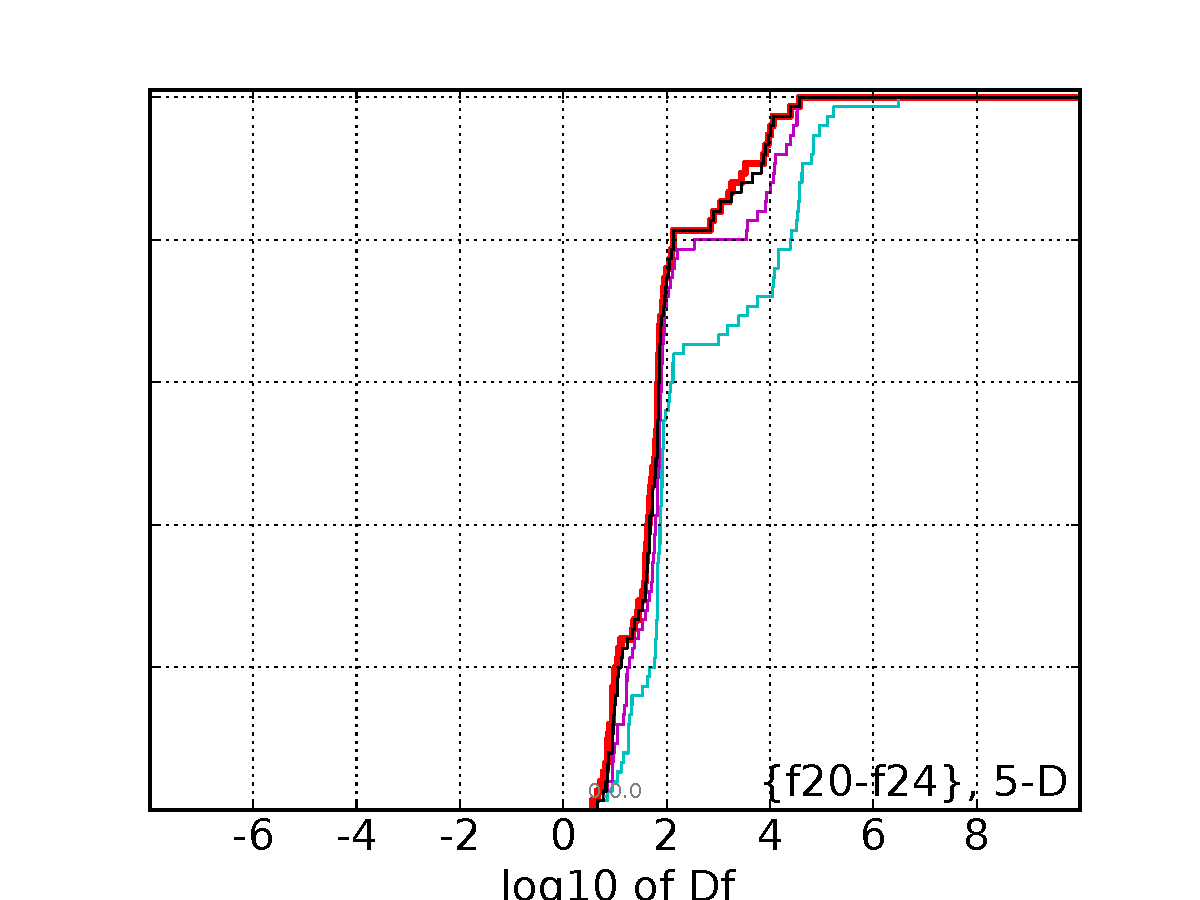
\includegraphics[width=0.2362\textwidth,trim=2.40cm 0 0 13mm, clip]{ppfvdistr_05D_mult2} &
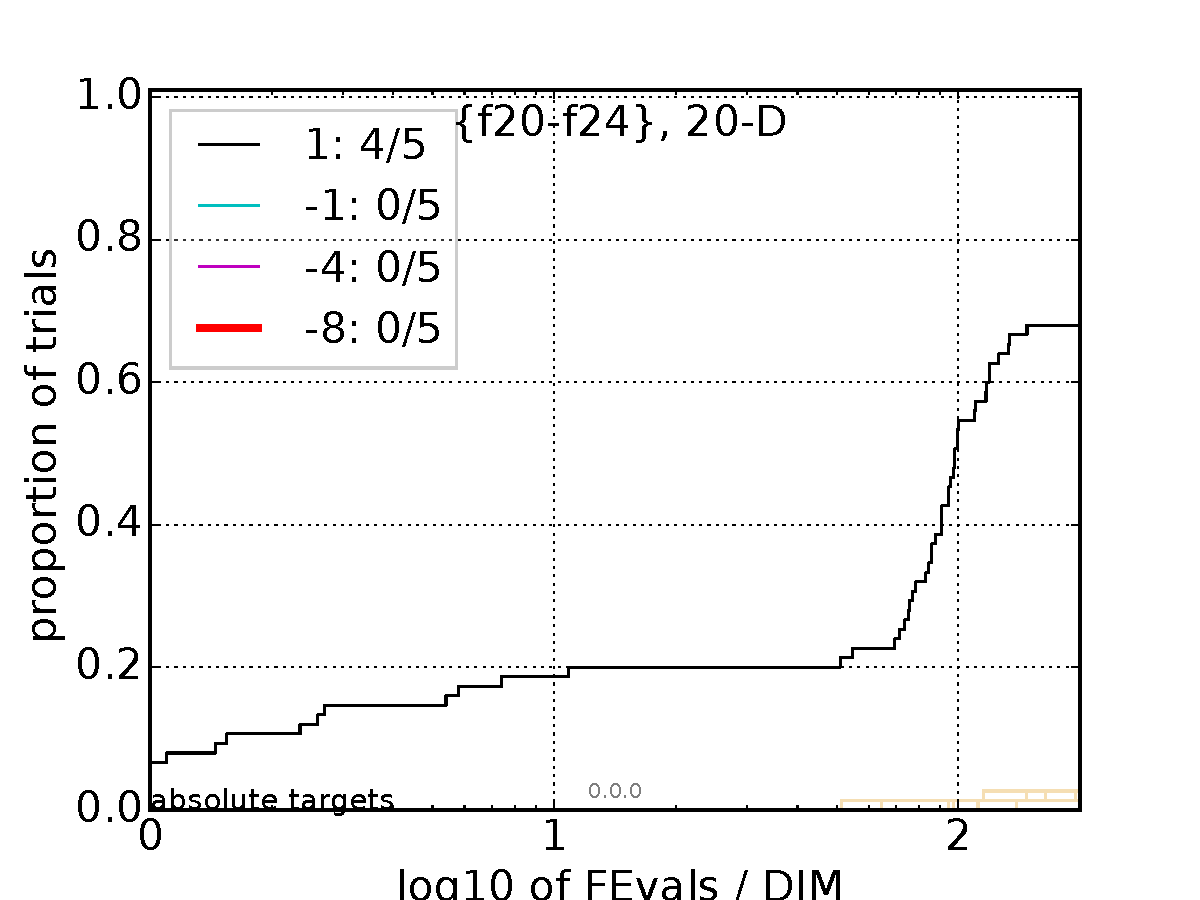
\includegraphics[width=0.268\textwidth,trim=0 0 0 13mm, clip]{pprldistr_20D_mult2} &
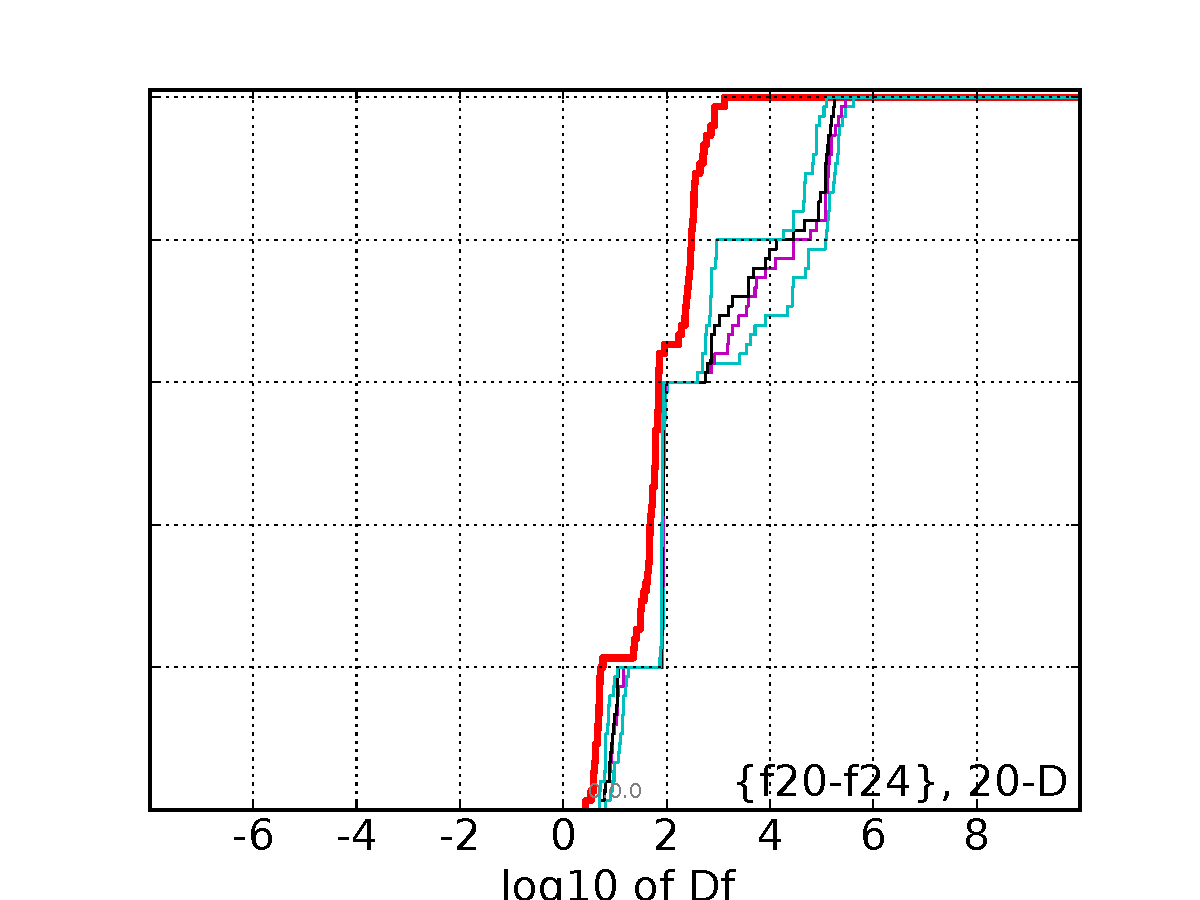
\includegraphics[width=0.2362\textwidth,trim=2.40cm 0 0 13mm, clip]{ppfvdistr_20D_mult2}\\[-2ex]
\rot{all functions}
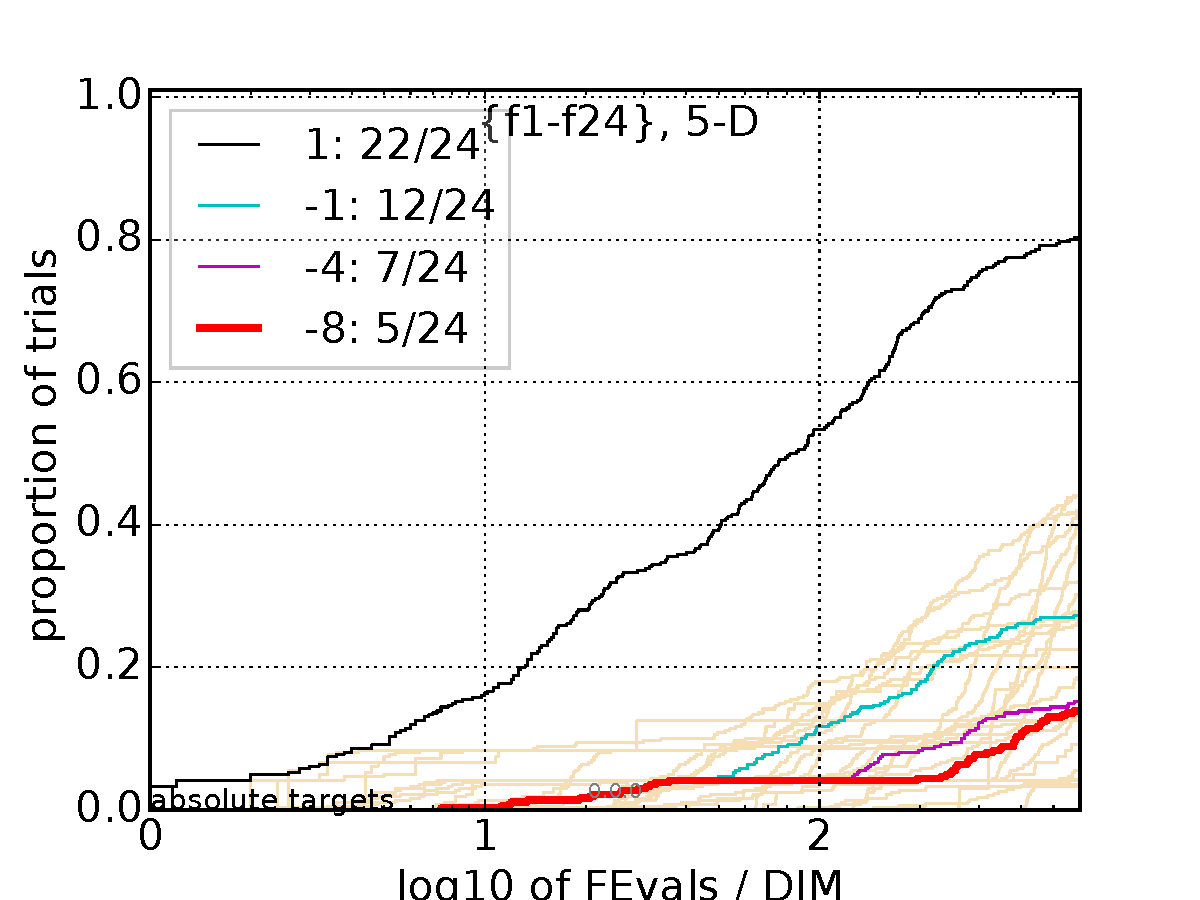
\includegraphics[width=0.268\textwidth,trim=0 0 0 13mm, clip]{pprldistr_05D_noiselessall} &
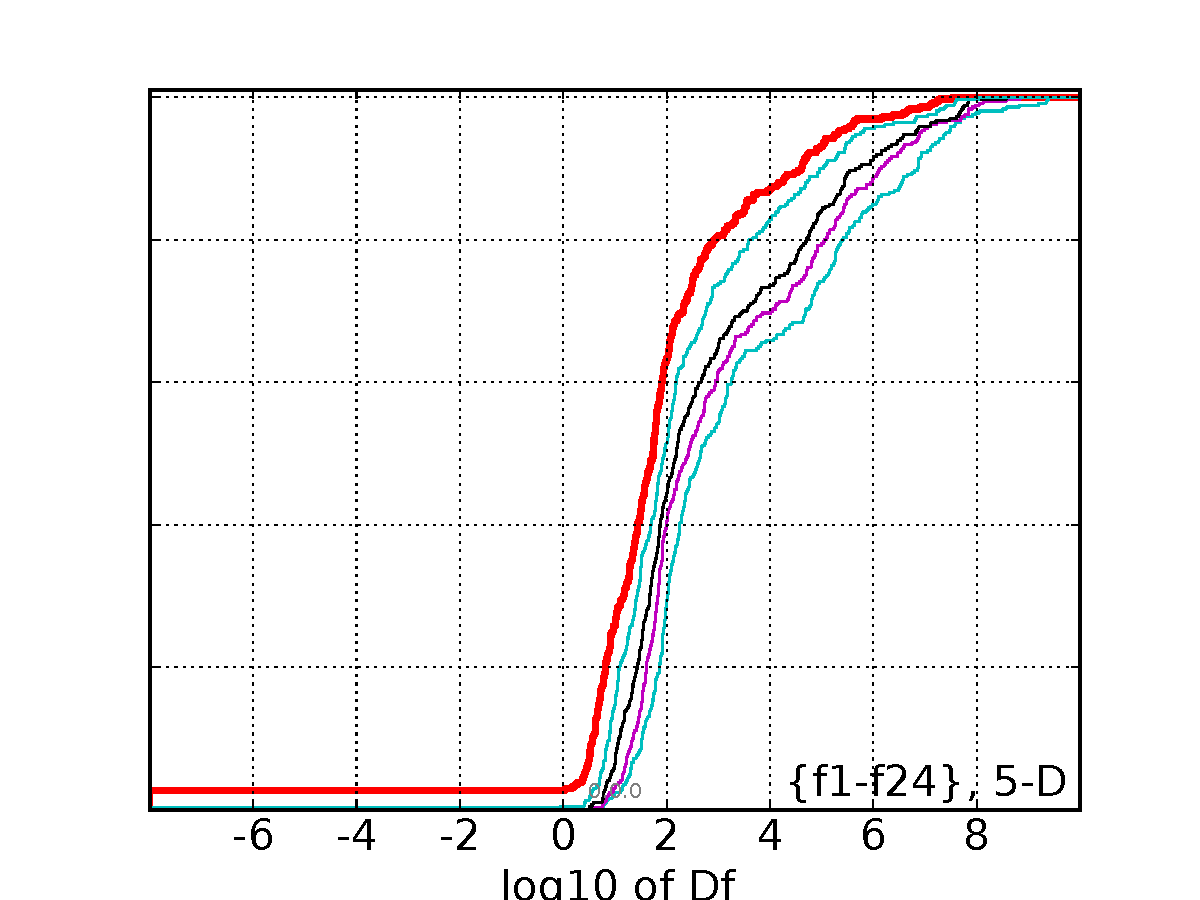
\includegraphics[width=0.2362\textwidth,trim=2.40cm 0 0 13mm, clip]{ppfvdistr_05D_noiselessall} &
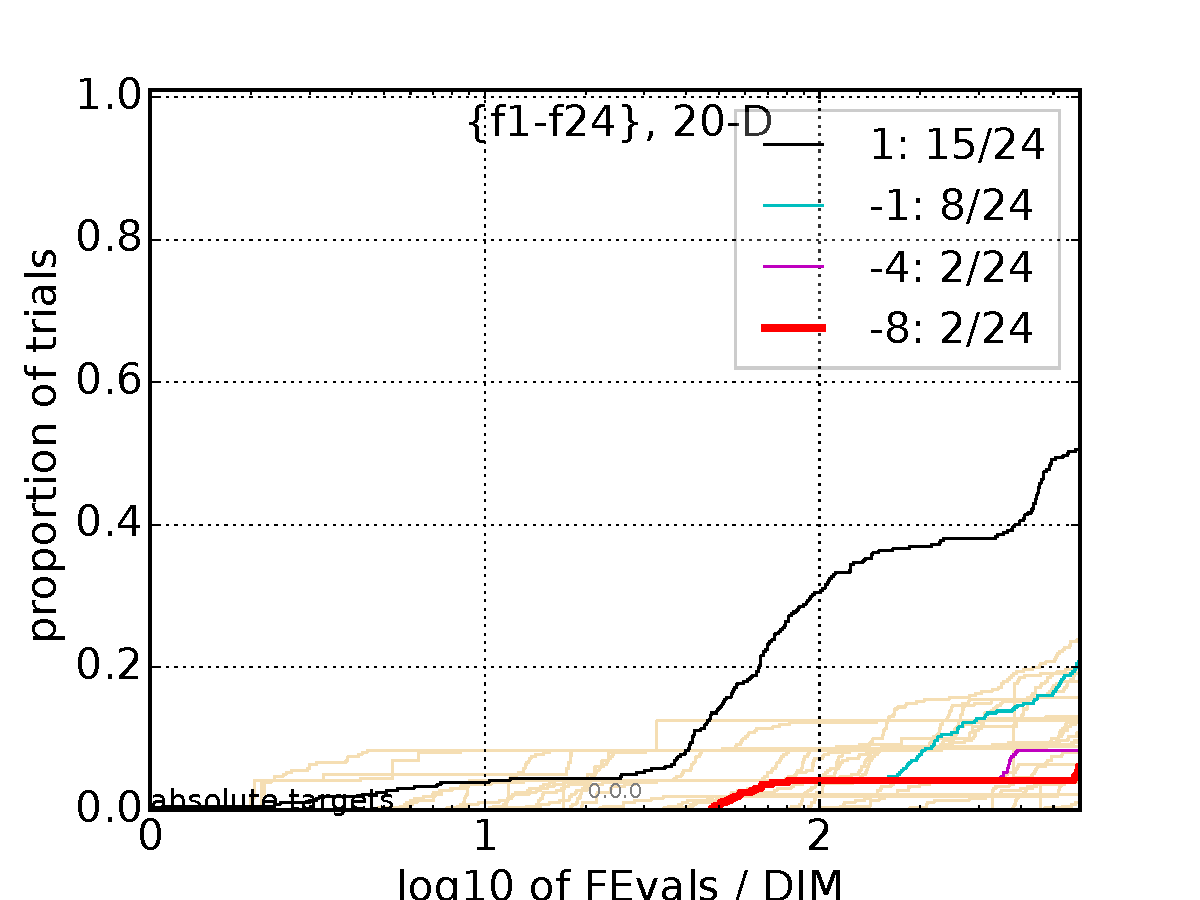
\includegraphics[width=0.268\textwidth,trim=0 0 0 13mm, clip]{pprldistr_20D_noiselessall} &
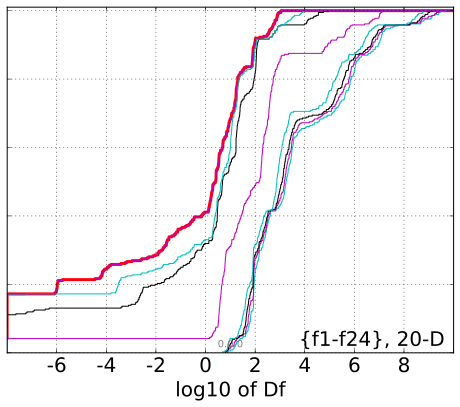
\includegraphics[width=0.2362\textwidth,trim=2.40cm 0 0 13mm, clip]{ppfvdistr_20D_noiselessall}
\vspace*{-0.5ex}
\end{tabular}
 \caption{\label{fig:RLDs}
 \bbobpprldistrlegend{}
 }
\end{figure*}
%%%%%%%%%%%%%%%%%%%%%%%%%%%%%%%%%%%%%%%%%%%%%%%%%%%%%%%%%%%%%%%%%%%%%%%%%%%%%%%


%%%%%%%%%%%%%%%%%%%%%%%%%%%%%%%%%%%%%%%%%%%%%%%%%%%%%%%%%%%%%%%%%%%%%%%%%%%%%%%
%%%%%%%%%%%%%%%%%%%%%%%%%%%%%%%%%%%%%%%%%%%%%%%%%%%%%%%%%%%%%%%%%%%%%%%%%%%%%%%

% aRT loss ratios (figure and table)

%%%%%%%%%%%%%%%%%%%%%%%%%%%%%%%%%%%%%%%%%%%%%%%%%%%%%%%%%%%%%%%%%%%%%%%%%%%%%%%
\begin{figure}
\centering
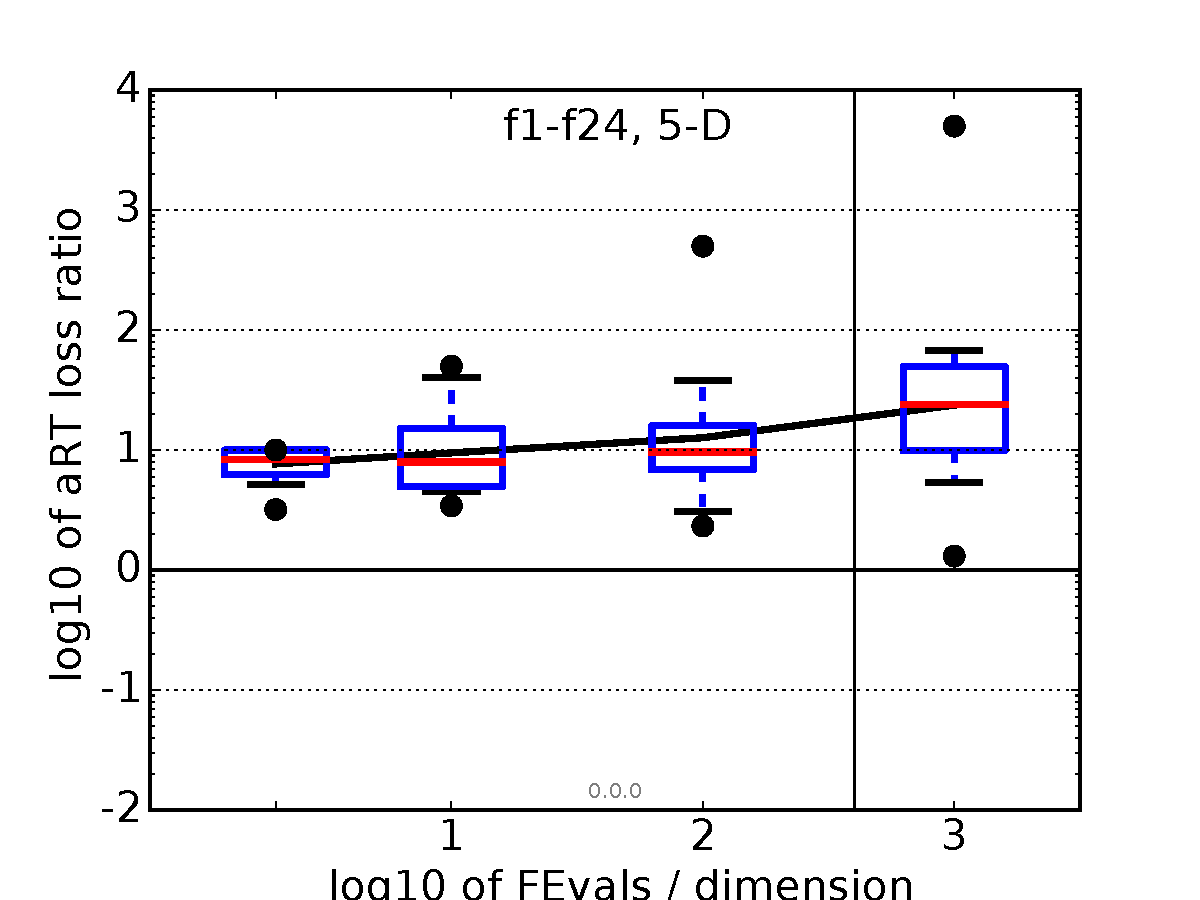
\includegraphics[width=0.24\textwidth,trim=0 0 16mm 12mm, clip]{pplogloss_05D_noiselessall}% 
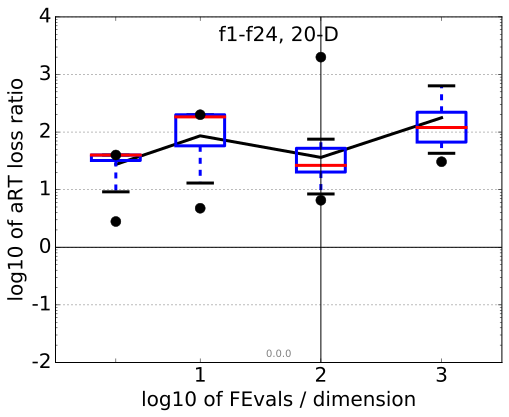
\includegraphics[width=0.24\textwidth,trim=7mm 0 9mm 12mm, clip]{pplogloss_20D_noiselessall}%
\\[-6.2ex]
\parbox{0.49\columnwidth}{\centering 5-D}%
\parbox{0.49\columnwidth}{\centering 20-D}\\[5ex]
%
\input{\bbobdatapath\algfolder pploglosstable_05D_noiselessall}\\
\input{\bbobdatapath\algfolder pploglosstable_20D_noiselessall}
\caption{\label{tab:aRTloss}%
\bbobloglosstablecaption{}
}
\end{figure}


%%%%%%%%%%%%%%%%%%%%%%%%%%%%%%%%%%%%%%%%%%%%%%%%%%%%%%%%%%%%%%%%%%%%%%%%%%%%%%%
%%%%%%%%%%%%%%%%%%%%%%%%%%%%%%%%%%%%%%%%%%%%%%%%%%%%%%%%%%%%%%%%%%%%%%%%%%%%%%%

% aRT loss ratios per function group

%%%%%%%%%%%%%%%%%%%%%%%%%%%%%%%%%%%%%%%%%%%%%%%%%%%%%%%%%%%%%%%%%%%%%%%%%%%%%%%
\begin{figure}
\begin{tabular}{@{}l@{}@{}l@{}}
\multicolumn{1}{c}{5-D} & \multicolumn{1}{c}{20-D}\\
%\rot{all functions}
%\hspace*{-2mm}
\rot{separable fcts}
\hspace*{-2mm}
\includegraphics[width=0.24\textwidth,trim=0 0 16mm 12mm, clip]{pplogloss_05D_separ} &
\includegraphics[width=0.24\textwidth,trim=7mm 0 9mm 12mm, clip]{pplogloss_20D_separ}\\[-2ex]
\rot[2]{moderate fcts}
\hspace*{-2mm}
\includegraphics[width=0.24\textwidth,trim=0 0 16mm 12mm, clip]{pplogloss_05D_lcond} &
\includegraphics[width=0.24\textwidth,trim=7mm 0 9mm 12mm, clip]{pplogloss_20D_lcond}\\[-2ex]
\rot[1.3]{ill-conditioned fcts}
\hspace*{-2mm}
\includegraphics[width=0.24\textwidth,trim=0 0 16mm 12mm, clip]{pplogloss_05D_hcond} &
\includegraphics[width=0.24\textwidth,trim=7mm 0 9mm 12mm, clip]{pplogloss_20D_hcond}\\[-2ex]
\rot[1.6]{multi-modal fcts}
\hspace*{-2mm}
\includegraphics[width=0.24\textwidth,trim=0 0 16mm 12mm, clip]{pplogloss_05D_multi} &
\includegraphics[width=0.24\textwidth,trim=7mm 0 9mm 12mm, clip]{pplogloss_20D_multi}\\[-2ex]
\rot[1.0]{weak structure fcts}
\hspace*{-2mm}
\includegraphics[width=0.24\textwidth,trim=0 0 16mm 12mm, clip]{pplogloss_05D_mult2} &
\includegraphics[width=0.24\textwidth,trim=7mm 0 9mm 12mm, clip]{pplogloss_20D_mult2}
\vspace*{-0.5ex}
\end{tabular}
 \caption{\label{fig:aRTlogloss}%
\bbobloglossfigurecaption{}
}
\end{figure}

%%%%%%%%%%%%%%%%%%%%%%%%%%%%%%%%%%%%%%%%%%%%%%%%%%%%%%%%%%%%%%%%%%%%%%%%%%%%%%%


%%%%%%%%%%%%%%%%%%%%%%%%%%%%%%%%%%%%%%%%%%%%%%%%%%%%%%%%%%%%%%%%%%%%%%%%%%%%%%%
%\section{Discussion}  % and or conclusion, summary...
%%%%%%%%%%%%%%%%%%%%%%%%%%%%%%%%%%%%%%%%%%%%%%%%%%%%%%%%%%%%%%%%%%%%%%%%%%%%%%%

%
% The following two commands are all you need in the
% initial runs of your .tex file to
% produce the bibliography for the citations in your paper.
\bibliographystyle{abbrv}
\bibliography{bbob}  % bbob.bib is the name of the Bibliography in this case
% You must have a proper ".bib" file
%  and remember to run:
% latex bibtex latex latex
% to resolve all references
% to create the ~.bbl file.  Insert that ~.bbl file into
% the .tex source file and comment out
% the command \texttt{{\char'134}thebibliography}.
%
% ACM needs 'a single self-contained file'!
%

\clearpage % otherwise the last figure might be missing
\end{document}
